% !TeX document-id = {627414bf-e7a2-4218-9269-f76848e4211f}
%%
%% F5 compiles the whole document, runs bibliography, etc
%% F6 compiles the document only once, tableofcontents may be not correct after running this
%% F8 run biber
%%
% !TeX program = lualatex
% !TeX TXS-program:quick = txs:///lualatex/[--shell-escape] | txs:///biber | txs:///lualatex/[--shell-escape] | txs:///lualatex/[--shell-escape] | txs:///view
% !TeX TXS-program:compile = txs:///lualatex/[--shell-escape] | txs:///view
% !BIB program = biber
% !TeX encoding = utf8
% !TeX spellcheck = de_DE
% !TeX root = thesis.tex

\documentclass[
english,
%german,
%standalone,
%final,
]{bama}

%Authors firstname, put a space behind the name
\firstname{Harshit}

%Authors lastname
\lastname{Vaishya}

%Type of thesis (Bachelorarbeit, Masterarbeit, Bachelor's Thesis, Master's Thesis)
\thesis{Master's Thesis}

%Course, EEI/IuK/MT/...
\course{Information and Communication Technology}

%Title of the work
\title{Development of a physiological sensor board to evaluate and transmit ECG data with hardware-accelerator, embedded AI and secure element}
\subtitle{Untertitel der Arbeit}

%Keywords saved in the metadata, put something like FPGA, SCPI, RADAR, ... (separate with ;)
\keywords{ECG; CNN; FILTERS; SECURE ELEMENT}

%Names of tutors/Betreuer/supervisors including titles (seperate with ;)
%Corresponding professor
%Prof. Dr.-Ing. Dr.-Ing. habil. Robert Weigel
%Prof. Dr.-Ing. Georg Fischer
%team leader and/or group leader if primary tutor is not Akademischer Rat*in
%https://www.lte.tf.fau.de/lehrstuhl/person/
%primary tutor
\supervisor{Prof. Dr.-Ing. Georg Fischer; Benedict Scheiner; Tobias Zech; Norman Pfeiffer} %seperate with ;

%Begin date of thesis (format corresponding to the chosen language)
\thesisbegin{01.01.2024}

%Same for the end
\thesisend{30.06.2024}

%Month and year when thesis is handed in
%required for financial stuff at the institute
\thesisendmonth{6} %number of the month without leading 0 (1-12)
\thesisendyear{2024}

%Abstract for pdf metadata. This abstract will be visible in the archive of LTE and is visible in the metadata of the pdf output file. Avoid TeX here.
\abstract{
	Lörem ipsüm dolor sit ämet, consetetur sadipscing elitr, sed diam nonumy eirmod tempor invidunt ut labore et dolore magna aliquyam erat, sed diam voluptua. At vero eos et accusam et justo duo dolores et ea rebum. Stet clita kasd gubergren, no sea takimata sanctus est Lorem ipsum dolor sit amet. Lorem ipsum dolor sit amet, consetetur sadipscing elitr, sed diam nonumy eirmod tempor invidunt ut labore et dolore magna aliquyam erat, sed diam voluptua. At vero eos et accusam et justo duo dolores et ea rebum. Stet clita kasd gubergren, no sea takimata sanctus est Lorem ipsum dolor sit amet. Lorem ipsum dolor sit amet, consetetur sadipscing elitr, sed diam nonumy eirmod tempor invidunt ut labore et dolore magna aliquyam erat, sed diam voluptua. At vero eos et accusam et justo duo dolores et ea rebum. Stet clita kasd gubergren, no sea takimata sanctus est Lorem ipsum dolor sit amet.
	\\
	Duis autem vel eum iriure dolor in hendrerit in vulputate velit esse molestie consequat, vel illum dolore eu feugiat nulla facilisis at vero eros et accumsan et iusto odio dignissim qui blandit praesent luptatum zzril delenit augue duis dolore te feugait nulla facilisi. Lorem ipsum dolor sit amet.
}

%define bibliography file containing references
%edit this file in editor or with tools like jabref
%references can be downloaded at ub.fau.de, ieeexplore.com and via the online tool in jabref, paste in jabref from clipboard is possible
%thesis with modern lte templates can be drag and dropped into jabref
\bibliography{bibliography/bibliography.bib}

%define your acronyms in this file
%defines acronyms of long version used in text
%reference them with \ac{LNA} to get the long version at first use
%more commands see here: https://ctan.org/pkg/acro
\DeclareAcronym{FAU}{
	short = FAU,
	long  = Friedrich-Alexander-Universität
}

\DeclareAcronym{MOSFET}{
	short = MOSFET,
	long  = Metal-Oxide-Semi\-conductor Field-Effect Tran\-sistor
}

\DeclareAcronym{FFT}{
	short = FFT,
	long  = Fast Fourier Transformation
}

\DeclareAcronym{LTE}{
	short = LTE,
	long  = Lehrstuhl für Technische Elektronik,
	long-plural-form = Lehrstühle für Technische Elektronik 	% Unnütz, zeigt nur, wie es geht
}

\DeclareAcronym{BA}{
	short = BA,
	short-plural = s,
	long = Bachelorarbeit,
	long-plural = en
}

\DeclareAcronym{MA}{
	short = MA,
	short-plural = s,
	long = Masterarbeit,
	long-plural = en
}

%define manual hyphenation if automatic does not work well
\hyphenation{Dynamik-bereich}

%header with packages for special use cases
% -----------------------------------------

%math stuff
%defines math symbols and fonts
%%% math mode
%%% ---------

\usepackage{mathtools}
\usepackage{unicode-math}
\usepackage{lualatex-math}	% Lädt einige Korrekturen für amsmath, mathtools und weitere.

%math font using unicode-math
\IfFontExistsTF{TeX Gyre Termes Math}{
	\setmathfont{TeX Gyre Termes Math}}{
	\setmathfont{texgyretermes-math.otf}}

%make normal text in math mode look like other text
\IfFontExistsTF{TeX Gyre Termes}{
	\setmathfont{TeX Gyre Termes}[range=\mathup/{latin,Latin,num,greek,Greek}]}{
	\setmathfont{texgyretermes-regular.otf}[range=\mathup/{latin,Latin,num,greek,Greek}]}

%custom mathematical symbols
\AtBeginDocument{%
	%upright partial derivation symbol
	\let\umathpartial\partial
	\renewcommand\partial{\symup\umathpartial}
	
	%upright letters for constants
	\newcommand\jj{\operatorname{j}}
	\newcommand\ii{\operatorname{i}}
	\newcommand\ee{\operatorname{e}}
	\newcommand\pipi{\uppi}
	\let\jmath\jj
	
	%upright integral d
	\newcommand\dd[1]{\,\operatorname{d}\!#1\xspace}
	
	%vector arrow
	\newcommand{\vect}[1]{\overrightarrow{#1}}
	
	%upright grad, div, rot
	\DeclareMathOperator{\grad}{grad}
	\DeclareMathOperator{\diver}{div}
	\DeclareMathOperator{\rot}{rot}
	
	%limits can be used with _ and ^ and are always placed above and unter the int sign
	\let\intold\int
	\removenolimits{\int}\removenolimits{\iint}\removenolimits{\iiint}
	\removenolimits{\oint}\removenolimits{\oiint}\removenolimits{\oiiint}
}

\usepackage{esint}

%numbers and units
\ifgerman{
	\usepackage[locale=DE, per-mode=symbol-or-fraction, detect-all=true]{siunitx}
}
\ifenglish{
	\usepackage[per-mode=symbol-or-fraction, detect-all=true]{siunitx}
}
\usepackage{icomma} %correct spacing in german mode


%code listings
%%% code listings
%%% -------------

% Farben definieren für package listings 
%\usepackage{color}
%\definecolor{middlegray}{rgb}{0.5,0.5,0.5}
%\definecolor{lightgray}{rgb}{0.8,0.8,0.8}
%\definecolor{orange}{rgb}{0.8,0.3,0.3}
%\definecolor{yac}{rgb}{0.6,0.6,0.1}
\definecolor{commentgreen}{rgb}{0,0.6,0.0}
\definecolor{keyred}{RGB}{127,0,85}

% Syntax highlighting
\usepackage{listings}
\usepackage{lstautogobble}
\lstset{
	basicstyle=\small\ttfamily,
	%keywordstyle=\bfseries\ttfamily\color{red},
	stringstyle=\color{purple}\ttfamily,
	commentstyle=\color{teal}\ttfamily, %comments in green
	numberstyle=\color{grey},
	showtabs=false,
	showspaces=false,
	showstringspaces=false,
	flexiblecolumns=false,
	tabsize=2,
	numbers=left, %line numbers
	numberstyle=\tiny,
	numberblanklines=true,
	stepnumber=1,
	numbersep=10pt,
	xleftmargin=15pt,
	breaklines=true, %line breaks
	breakatwhitespace=true,
	autogobble=true, %autoremove indention
} 


%%% figures
%%% -------

\usepackage{float}
\usepackage{wrapfig}
%\usepackage[hyperref=false]{scrhack} %solves komascript incompatibilities
%\usepackage[countmax]{subfloat}
\usepackage[section]{placeins} %ensure figures are in the correct section
%\usepackage[format=hang]{caption}
\usepackage{subcaption} %allow figures with subfigures

% Standardargument für Platzierung von figures und tables kann hier global mit absteigender Priorität eingestellt werden.
% Vorgabe: tbp (1. oben, 2. unten, 3. eigene Seite)
% Weitere Möglichkeiten: h (hier), H (unbedingt hier)
\makeatletter
\renewcommand{\fps@figure}{htbp}
\renewcommand{\fps@table}{htbp}  
\makeatother
% Ende Spezialanpassung figures


%packages for graphics created in LaTeX
%standalone, tikz, pgfplots
%%% Tikz drawings
%%% ------------

\usepackage[mode=tex]{standalone}
%\usepackage[mode=buildnew]{standalone}

\usepackage{tikz}
\usepackage{tikzsymbols}
\usepackage[european,cuteinductors]{circuitikz}
\usetikzlibrary{calc,arrows,patterns}

% pgfplot
\usepackage{pgfplots}
\usepgfplotslibrary{smithchart}
\usepgfplotslibrary{groupplots}

%\pgfplotsset{compat=1.10}
%\pgfplotsset{every tick label/.style={font={\scriptsize}}}
%\pgfplotsset{every axis label/.style={font={\small}}}
%\pgfplotsset{every legend /.style={font={\boldmath\small\bfseries}}}
%\pgfplotsset{every label/.style={font={\boldmath\small\bfseries}}}

\pgfplotsset{width=.8\textwidth}
\pgfplotsset{height=.5\textwidth}
\pgfplotsset{grid=both}
\pgfplotsset{major tick style={thin,black}}% modifies the style ‘every tick’
\pgfplotsset{minor tick style={very thin,black}}% modifies the style ‘every tick’
\pgfplotsset{major grid style={thin}} %modifies the style ‘every major grid’
\pgfplotsset{minor grid style={very thin}} % modifies the style ‘every minor tick’
%\pgfplotsset{minor x tick num=1} %n minor ticks zwischen major ticks(major tiks müssen selben abstand haben) (problems with smithchart)
%\pgfplotsset{minor y tick num=1} %n minor ticks zwischen major ticks(major tiks müssen selben abstand haben) (problems with smithchart)
%\pgfplotsset{xlabel near ticks,ylabel near ticks}
%For ylabel offsets:

%For ylabel offsets:
\pgfplotsset{ylabsh/.style={every axis y label/.style={at={(0,0.5)}, xshift=#1, rotate=90}}}
\pgfplotsset{xlabsh/.style={every axis x label/.style={at={(0.5,0)}, yshift=#1}}}
\pgfplotsset{filter discard warning=false}%disable filter warning using "each nth point"

\pgfplotsset{every axis/.append style={line width=1pt}}

%cycle list für plots, !!!! \addplot+ verwenden!
%\pgfplotsset{
%	cycle list={
%		blue,
%		red,
%		{black, thick, dashed},
%		violet
%	}
%} 


\begin{document}
	%roman page numbering, etc..	
	\frontmatter
	
	%title page
	\maketitle
	
	%declaration of own work...
	\declaration
	
	%summary of the work
	%(not as much result orientated as the summary at the end)
	% !TeX root = ../thesis.tex

%German abstract, optional for thesis written in english
\ifgerman{
	\chapter*{Kurzfassung}
	\label{sec:kurzfassung}

	Lorem ipsum dolor sit amet, consetetur sadipscing elitr, sed diam nonumy eirmod tempor invidunt ut labore et dolore magna aliquyam erat, sed diam voluptua. At vero eos et accusam et justo duo dolores et ea rebum. Stet clita kasd gubergren, no sea takimata sanctus est Lorem ipsum dolor sit amet. Lorem ipsum dolor sit amet, consetetur sadipscing elitr, sed diam nonumy eirmod tempor invidunt ut labore et dolore magna aliquyam erat, sed diam voluptua. At vero eos et accusam et justo duo dolores et ea rebum. Stet clita kasd gubergren, no sea takimata sanctus est Lorem ipsum dolor sit amet. Lorem ipsum dolor sit amet, consetetur sadipscing elitr, sed diam nonumy eirmod tempor invidunt ut labore et dolore magna aliquyam erat, sed diam voluptua. At vero eos et accusam et justo duo dolores et ea rebum. Stet clita kasd gubergren, no sea takimata sanctus est Lorem ipsum dolor sit amet.

	Duis autem vel eum iriure dolor in hendrerit in vulputate velit esse molestie consequat, vel illum dolore eu feugiat nulla facilisis at vero eros et accumsan et iusto odio dignissim qui blandit praesent luptatum zzril delenit augue duis dolore te feugait nulla facilisi. Lorem ipsum dolor sit amet.
}

% English abstract, required for german and english thesis language
\chapter*{Abstract}
\label{sec:abstract}

Ischemic heart diseases are currently a leading cause of mortality worldwide, responsible for approximately 16\% of total global deaths. This underscores the importance of timely detection of heart rate variabilities in reducing mortality rates. Current techniques for detecting heart rate variabilities involve extracting RAW ECG data and transmitting it to remote or cloud servers for further analysis. However, this approach is inconvenient for continuous monitoring as it results in significant power consumption.

\vspace{1em}

\noindent Over the past decade, the \ac{IoT} has become increasingly integrated into our daily lives. Everything from TVs, speakers, and toys, to appliances is now connected to the internet. With the rapid increase in \ac{IoT} data and the emergence of AI, there's an opportunity for edge intelligence. Integrating edge AI with IoT can bring additional benefits to systems, such as reduced power consumption, lower latency, bandwidth optimization, and enhanced data security.

\vspace{1em}

\noindent Designing an end-to-end device for recording \ac{ECG} and predicting heart rate variability on the edge, while ensuring user data security through encryption, is the focus of this thesis. In this regard, a simple, cost-efficient analog circuit PCB is designed to detect the R-peaks of ECG, and a method for translating and deploying neural network models on embedded devices using MAX78000 APIs is presented. Additionally, a secure element is interfaced with the device to enhance its safety features. 

\vspace{1em}


\noindent The extracted ECG signals are further compared with off-the-shelf ECG Holter monitors in terms of R-peak detection. Furthermore, a comparison is made in terms of power and energy consumption between transmitting ECG raw data to a remote server via Bluetooth and performing edge computation for heart rate variability detection.

	
	%table of contents including heading
	\tableofcontents
	
	%table with acronyms specified in the acronyms file and used in thesis
	\printacronyms
	
	%arabic page numbering
	\mainmatter
	
	%demonstration of LaTeX capabilities

	
	
	
	%content of the thesis splitted in several chapters
	
	%Introduction
	%
	%What is it all about?
	%Motivation, context, task definition, own approach
	% !TeX root = ../thesis.tex

\chapter{Introduction}
\label{chap:introduction}

The development of the first ECG machine in the Netherlands by Willem Einthoven marked the beginning of a revolution in monitoring cardiac activity. As of 2023, cardiovascular diseases, particularly \ac{IHD}, are among the top \ac{NCDs} , resulting in approximately 18 million deaths worldwide annually~\cite{who2023}. Cardiac arrhythmias, which include conditions such as premature ventricular and atrial contractions, \ac{AF}, ventricular fibrillation, and atrial flutter, are common and significant due to their association with increased risk of severe cardiovascular events like strokes, heart failure, and coronary artery disease~\cite{sharma2018, liu2021}. Atrial fibrillation, in particular, is a leading cause of mortality as it complicates the detection and management of cardiovascular conditions~\cite{liu2021}. \ac{ECG} play a crucial role in the diagnosis and management of arrhythmias, using waveforms to provide essential first-hand information on cardiac function under various conditions. Timely and accurate ECG monitoring is thus critical for the effective treatment of cardiovascular diseases.

\section{Motivation}

\subsection{Diagnostic Challenges and Limitations of Traditional ECG Monitoring}

Since Einthoven's pioneering work, ECG technology has undergone substantial evolution. However, the 12-lead ECG system remains the gold standard for recording cardiac waveforms. This system uses ten electrodes: six are placed on the chest (V1 to V6) and four on the limbs. Depending on the electrode combination, twelve different lead signals can be captured for diagnosing conditions such as atrial fibrillation~\cite{liu2021}. Traditionally, these 12-lead ECGs have been instrumental in diagnosing AF, requiring skilled physicians to record and interpret the results accurately. However, AF can often be asymptomatic, making it challenging to detect since symptoms may not be present during standard ECG tests~\cite{page2003}. Additionally, the intermittent nature of AF necessitates extended monitoring, which is impractical with the cumbersome 12-lead setup due to discomfort and complexity, especially for long-term wear~\cite{liu2021}. Consequently, this reliance on healthcare professionals for interpretation also delays timely intervention, making the process expensive and logistically challenging for many patients.

\subsection{The Evolution of IoT and Continuous Monitoring in Cardiac Care}

The integration of \ac{IoT} technologies in healthcare represents a significant advancement in medical monitoring. IoT-enabled ECG systems are now capable of continuously sensing cardiac signals and transmitting the raw data to cloud-based or remote servers for further analysis. This shift has the potential to automate the detection of AF using advanced machine learning algorithms, substantially reducing the time and cost associated with traditional diagnostic methods. However, these systems often rely on high-energy-consumption wireless communication technologies such as Zigbee and Bluetooth, leading to devices that are power-intensive and not ideal for continuous, long-term monitoring~\cite{muhoza2023}.

\subsection{Advancing ECG Architecture with Embedded Edge AI}

The pursuit of personalized medicine increasingly demands technologies that enable reliable, comfortable, and affordable monitoring of heart activity in everyday settings. Addressing the challenges of power consumption and patient comfort requires advancing the medical sensing architecture. Recent advancements in microcontroller capabilities and the advent of sophisticated deep learning algorithms allow for running compact AI models directly on microcontrollers~\cite{muhoza2023}. This study aims to develop a cost-effective, two-electrode (single-lead) ECG system for efficient R peak detection, which simplifies continuous monitoring. Furthermore, by leveraging edge AI technology, the system can locally process data to detect abnormalities in real time, thereby reducing power consumption and enhancing the feasibility of long-term cardiac health monitoring.

\section{Scope of the Thesis}

This thesis focuses on developing a physiological sensor board for the acquisition of ECG signals and classifying heart abnormalities at the edge. The project aims to provide a simple and cost-efficient method for acquiring ECG signals, enhancing the security and usability of ECG monitoring, and detecting abnormalities through the integration of hardware-accelerated embedded AI and a secure element. This thesis proposes a new architecture that can significantly improve medical sensing technology, making the sensing process easier, faster, and more power-efficient.

\subsection{Detailed Objectives}

\begin{itemize}
	\item \textbf{ECG System Development:} The thesis designed a compact, two-electrode ECG system optimized for user comfort and simplicity, making it suitable for long-term continuous monitoring.
	\item \textbf{Embedded AI Integration:} Embedded \ac{AI} was implemented using the Maxim78000 platform to process ECG data on-device, reducing dependency on remote processing and aiming to improve the speed and reliability of cardiac abnormality detection.
	\item \textbf{Security Implementation:} The Infineon OPTIGA Trust M secure element was utilized to ensure all patient data is encrypted, addressing the critical need for privacy and security in healthcare applications.
	\item \textbf{Energy Efficiency Analysis:} The system's power consumption was evaluated and optimized to extend battery life, which is essential for continuous monitoring applications.
\end{itemize}

\subsection{Delimitation}

The research focused on the development and initial testing of the ECG monitoring system within a lab environment and did not include commercial product development or explore the regulatory aspects of medical device approval.

\section{Outline of the Thesis}

This thesis is organized into the following chapters:

\begin{enumerate}
	\item \textbf{Chapter 1: Introduction} \\
	Introduces the research background, problem statement, objectives, and scope of the thesis.
	\item \textbf{Chapter 2: Literature Review} \\
	Reviews the physiological generation of heart signals, existing technologies, methodologies, and different architectures used in ECG monitoring. It also examines microcontrollers capable of running edge AI algorithms, comparing their energy consumption and computational capabilities, and discusses the importance of security in medical sensing.
	\item \textbf{Chapter 3: System Design and Development} \\
	Discusses the hardware and software design architecture of the complete physiological sensor board for ECG, covering everything from PCB design—including circuit design, filter design, \ac{ADC} conversion, data transfer—to component selection and integration of the Maxim78000 edge AI and Infineon secure element.
	\item \textbf{Chapter 4: Implementation and Testing} \\
	Describes the experimental setup and methodologies used for performance and security testing, detailing the implementation of the neural network on the Maxim78000 and the integration steps involved.
	\item \textbf{Chapter 5: Results and Discussion} \\
	Presents experimental results and analyzes the performance of the system in terms of energy efficiency, power consumption, and accuracy. It discusses the findings in the context of existing technologies and the theoretical framework established in earlier chapters.
	\item \textbf{Chapter 6: Conclusions and Future Work} \\
	Summarizes the research, evaluates the achievements relative to the original goals, and suggests future research directions to further enhance the system’s capabilities.
\end{enumerate}

	
	% !TeX root = ../thesis.tex

\chapter{Literature Survey}
\label{chap:literature_survey}

In this chapter, we will provide the background knowledge of the topic that was presented in Chapter 1. We will begin with an overview of the historical milestones of ECG and then move on to understand the basic knowledge of the cardiac cycle and the generation of ECG. We will then focus on understanding various ECG acquisition methods, emphasizing the advancement from multi-lead to single-lead technology. Next, we will explore the key challenges, such as noise interference, and discuss how edge computing and artificial intelligence have started to transform ECG monitoring, enhancing both performance and security. Finally, we will focus on the integration of edge computing on microcontrollers and explore different microcontrollers that can perform edge computing in terms of energy and operation. This review sets the stage for subsequent chapters highlighting challenges and emerging solutions in this field.

\section{Basic Knowledge of ECG}
\vspace{1em}
\subsection{Historical Development of ECG Technology}
\vspace{1em}
The study of phenomena such as the electric discharge of cramp fish and thunderstorms has been documented for many centuries. In 1781, Luigi Galvani made a groundbreaking discovery during a frog dissection. He observed that electrical stimulation of frog nerves resulted in muscle contraction, a phenomenon he termed "animal electricity." This discovery laid the biological foundations of electrophysiology for the first time~\cite{yang2015}.\\


\noindent Galvani's findings captured the attention of the scientific community. However, it was not until 1856 that Köllicker and Müller observed that the heart muscle itself could generate electrical activity. This observation was furthered nearly a decade later when, between 1869 and 1870, Alexander Muirhead recorded the first electrocardiogram (ECG) in London using a siphon instrument. Subsequently, in 1887, Augustus Waller used a capillary electrometer to record the heart's electrical activity~\cite{johansson2001}.\\

\noindent The significant advancement in ECG technology came from Dutch physiologist Willem Einthoven, who is often hailed as the father of electrocardiography. In 1893, Einthoven introduced the term "electrocardiography" into medical terminology. His major breakthrough occurred in 1901 with the invention of the string galvanometer, which revolutionized the recording of ECGs, as depicted in figure \ref{fig:einthoven_machine} . Furthermore, Einthoven simplified the electrode setup from the initially proposed five electrodes to just three. These electrodes were used to form the three standard leads, which facilitated the creation of Einthoven's triangle. This concept remains a fundamental part of ECG measurements today. Einthoven's dedication to advancing electrocardiography continued for over 25 years, culminating in him being awarded the Nobel Prize in 1924 for his contributions to medical science~\cite{alghatrif2012}~\cite{yang2015}

\begin{figure}[tb]
	\centering
	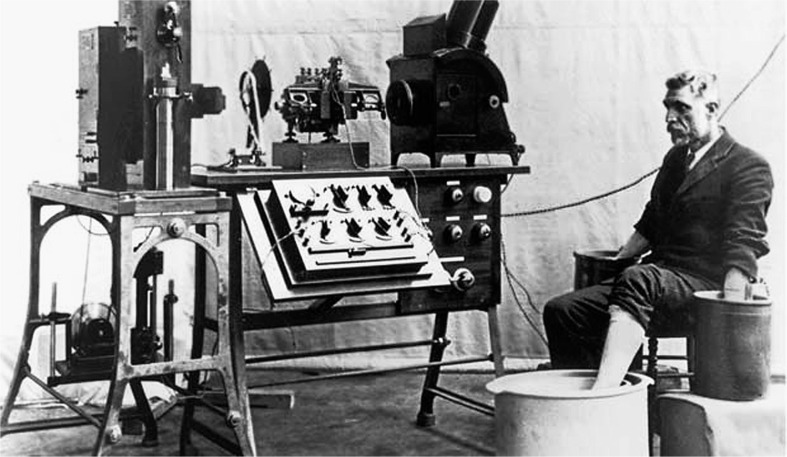
\includegraphics[width=0.8\textwidth]{images/einthoven_machine}
	\caption{Old string galvanometer electrocardiography~\cite{alghatrif2012}}
	\label{fig:einthoven_machine}
\end{figure}

\vspace{1em}

\noindent Despite numerous advancements and refinements in recording electrical potentials from the body's surface since Einthoven's string galvanometer, the fundamental principles of electrocardiography have remained largely unchanged.
\vspace{1em}


\subsection{Understanding the Cardiac Cycle}
\vspace{1em}
\noindent The heart comprises four chambers: the right and left atria, and the right and left ventricles. It also includes four valves: the tricuspid valve between the right atrium and ventricle, the mitral valve between the left atrium and ventricle, the pulmonary valve located between the right ventricle and the pulmonary artery, and the aortic valve situated in the outflow tract of the left ventricle, which controls blood flow to the aorta \cite{malminen1995} (as shown in Figure \ref{fig:heart_anatomy}).\\

\begin{figure}[tb]
	\centering
	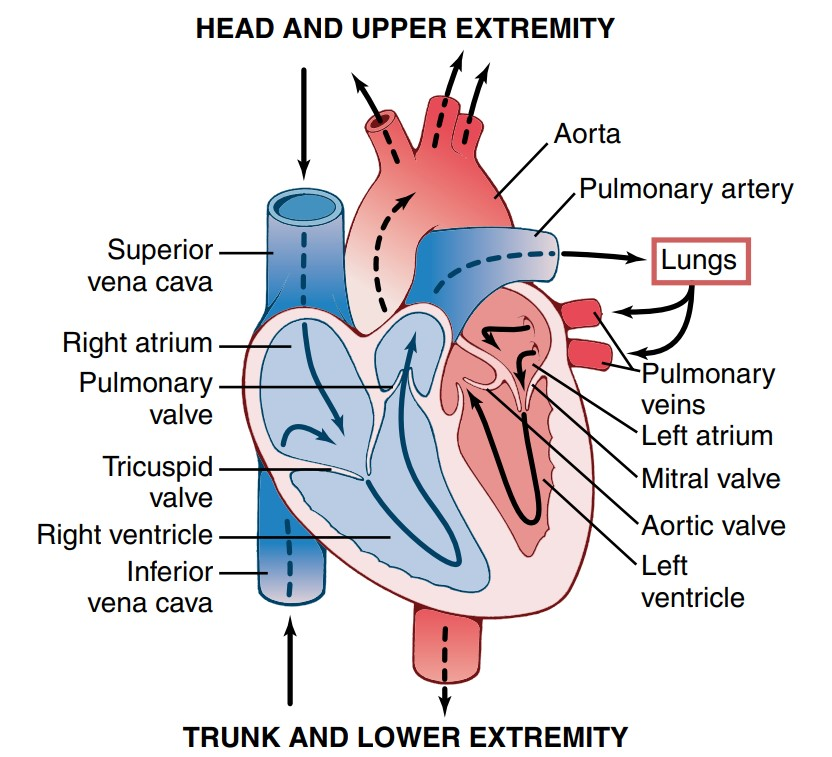
\includegraphics[width=0.8\textwidth]{images/anatomy of heart}
	\caption{Anatomy of the Heart~\cite{hall2015}}
	\label{fig:heart_anatomy}
\end{figure}


\noindent The cardiac cycle encompasses the events occurring from the beginning of one heartbeat to the beginning of the next. Blood distribution throughout the body is facilitated by the circulatory system, which includes two primary circuits: the pulmonary and the systemic circuits. The pulmonary circuit transports oxygen-deficient blood from the heart to the lungs and returns oxygenated blood to the heart, while the systemic circuit sends CO\textsubscript{2}-rich blood from the body to the heart and circulates oxygen-rich blood back to the body.\\

\noindent The cycle initiates on the right side of the heart, where deoxygenated blood enters the right atrium via the superior and inferior vena cavae. Upon contraction of the right atrium, blood flows through the tricuspid valve into the right ventricle. Once the right ventricle is filled, the tricuspid valve closes to prevent backflow into the atrium. The right ventricle then contracts, opening the pulmonary valve and pumping blood into the pulmonary artery to the lungs for oxygenation. After the blood is oxygenated in the lungs, it returns to the left atrium via the pulmonary veins.\\

\noindent Oxygenated blood is then drawn into the left ventricle through the mitral valve as the left atrium contracts. When the left ventricle is filled, the mitral valve closes to prevent backflow. Subsequent contraction of the left ventricle opens the aortic valve, allowing blood to be pumped into the aorta and distributed throughout the body. Following this, the aortic valve closes to prevent backflow to the left ventricle, which then relaxes in preparation for the next cycle of blood intake. This process constitutes one complete cardiac cycle \cite{hall2015, malminen1995}.


\subsection{Principles of ECG Signal Generation}
\vspace{1em}
\noindent A cardiac cycle is divided into two phases: diastole, a period of relaxation during which the heart fills with blood, and systole, a period of contraction. Diastole, also known as the re-polarization phase, involves the restoration of the cell's resting potential primarily through the efflux of potassium ions. Conversely, systole, or the depolarization phase, occurs when the cell becomes less negative relative to its resting state due to the influx of sodium ions through ion channels \cite{hall2015}.\\

\noindent The electrical activity in the heart originates from the sinoatrial (SA) node, located at the junction of the superior vena cava and the right atrium. Cells within the SA node are self-excitatory, often referred to as pacemaker cells, and typically initiate heartbeats at a rate of approximately 70 beats per minute. From the SA node, the electrical impulse spreads throughout the atria, causing atrial systole or depolarization. This impulse cannot directly reach the ventricles due to a fibrous septum that acts as an electrical insulator between the atria and ventricles. Thus, the transmission of the impulse from the atria to the ventricles is mediated by the atrioventricular node (AV node) through inter-nodal pathways. The AV node slows down the impulse, ensuring that atrial contraction completes before ventricular contraction begins, preventing simultaneous contraction of both chambers.\\

\noindent Following the AV node, the impulse travels through the bundle of His, which divides into left and right branches serving each ventricle. This conduction pathway extends into the Purkinje fibers, which distribute the impulse to the ventricular endocardial walls. As the electrical activity spreads from the inner to the outer walls of the ventricles, it triggers ventricular systole. Once all regions of the ventricular muscle have depolarized, they subsequently re-polarize.

\begin{figure}[h]
	\centering
	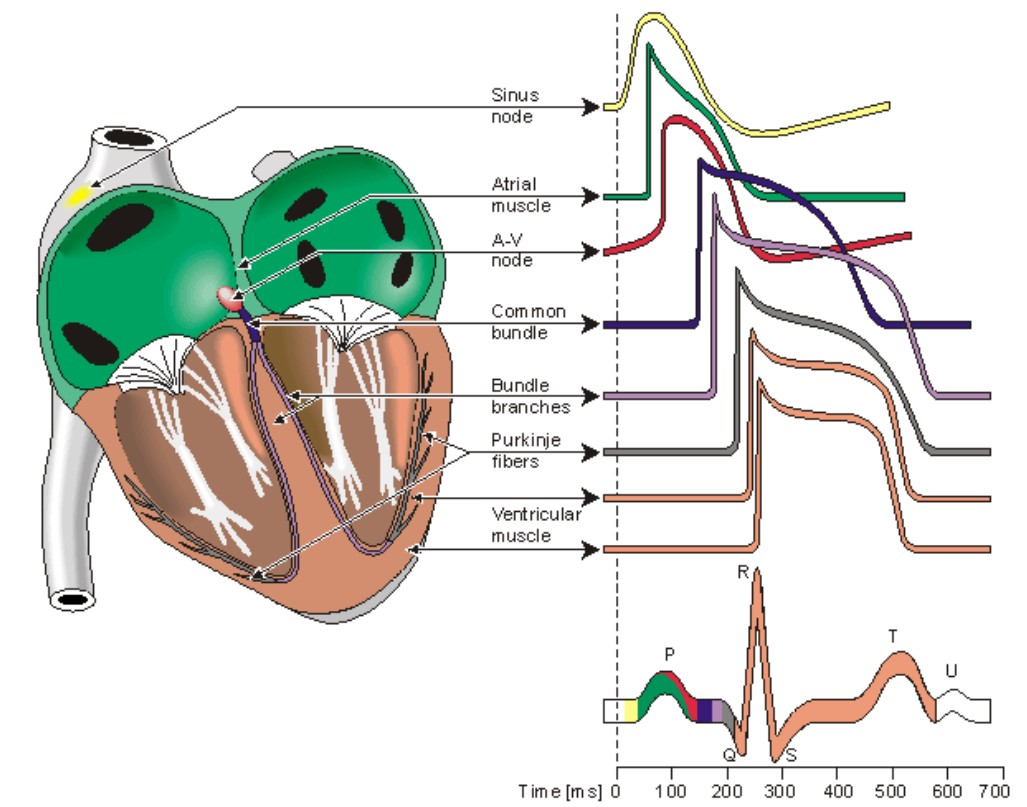
\includegraphics[width=0.8\textwidth]{images/action potention propagation of the heart}
	\caption{Waveform generated by the propagation of electrical signals through various specialized cardiac tissues, from the SA node to the ventricles~\cite{malminen1995}}
	\label{fig:ecg_signal}
\end{figure}

\noindent The ECG signal observed is essentially a superposition of action potentials from each cardiac tissue, demonstrating that the ECG is a composite of signals across different frequencies \cite{malminen1995}. This composite nature of the ECG signal helps in diagnosing various cardiac abnormalities by analyzing the waveform patterns.\\

\subsection{ECG Waveform}
\vspace{1em}
\noindent The resultant ECG signal consists of three principal waveforms:

\begin{itemize}
	\item \textbf{P wave:} This waveform results from the action potentials generated during the depolarization of the atria, which occurs just before atrial contraction begins.
	\item \textbf{QRS complex:} Comprising three individual waves—Q, R, and S—this complex is produced by the potentials generated during ventricular depolarization, just before the ventricles contract. Both the P wave and the QRS complex represent depolarization waves.
	\item \textbf{T wave:} Known as the repolarization wave, the T wave is generated as the ventricles recover from the state of depolarization.
\end{itemize}

\begin{figure}[h]
	\centering
	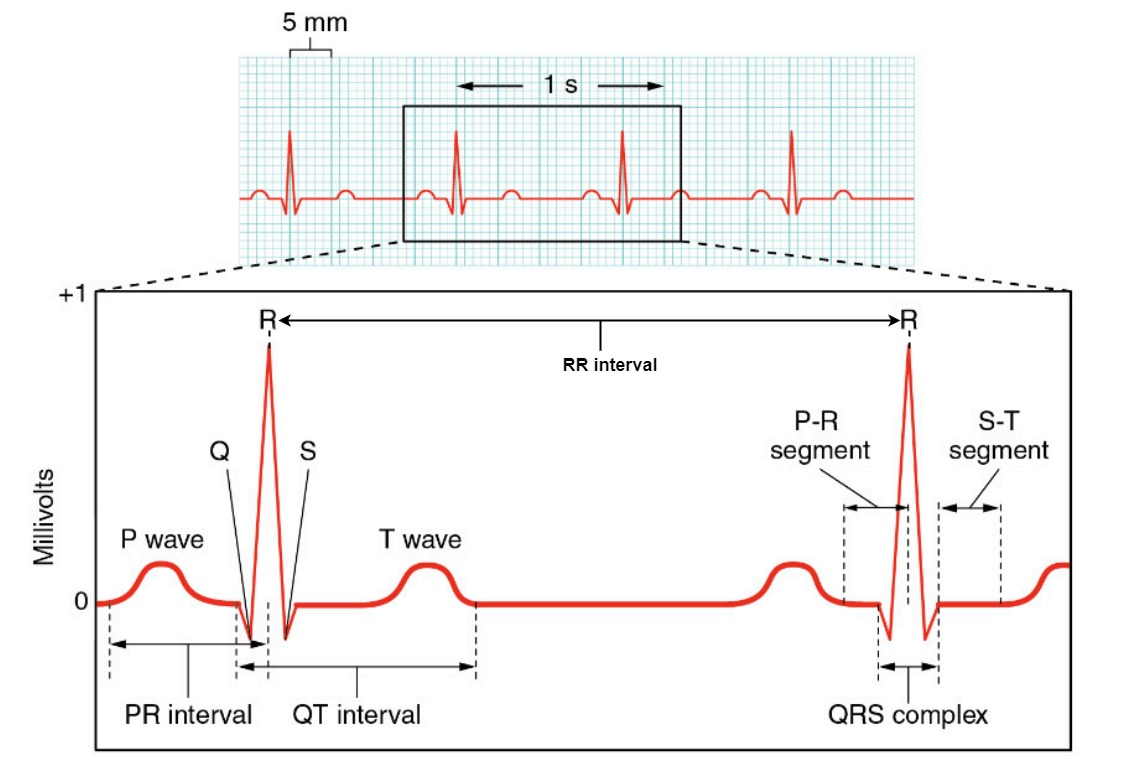
\includegraphics[width=0.8\textwidth]{images/temp}
	\caption{Illustrates a normal ECG signal, highlighting various intervals and signal markings that are crucial for understanding the heart's morphology~\cite{mamun2022}.}
	\label{fig:normal_ecg}
\end{figure}

\noindent The table \ref{tab:ecg_waves} below specifies the typical frequency and amplitude values for each type of ECG waveform:

\begin{table}[h]
	\centering
	\caption{Characteristics of ECG Waves\cite{zyout2023}}
	\begin{tabular}{|l|l|l|}
		\hline
		\textbf{ECG Wave} & \textbf{Amplitude} & \textbf{Frequency} \\ \hline
		P wave & 0.25 mV & 5-30 Hz \\ \hline
		QRS complex & 1.6 mV (R peak) & 8-50 Hz \\ \hline
		T wave & 0.1-0.5 mV & 0-10 Hz \\ \hline
	\end{tabular}
	\label{tab:ecg_waves}
\end{table}

\noindent In this thesis, the detection of atrial fibrillation—specifically through heart rate variability—is centered on identifying R peaks within the frequency range of 8-50 Hz, with peak power occurring in the range of 4 to 12 Hz \cite{murthy1978}.\\

\section{ECG Acquisition Techniques}
\vspace{1em}
\noindent Electrical activities of the heart can be detected on the skin using electrodes. An ECG machine captures these activities and graphically displays them, showing the heart's electrical potential or voltage as it fluctuates throughout a cardiac cycle.\\

\subsection{Three-Lead ECG Systems}\label{einthoven}
\vspace{1em}
\noindent The three-lead ECG system operates based on the principles first introduced by Willem Einthoven, who developed the concept of the three bipolar limb leads (I, II, and III). These leads form what is known as Einthoven's Triangle, a fundamental setup in the field of electrocardiography, as illustrated in Figure~\ref{fig:einthoven_triangle}.

\begin{figure}[h]
	\centering
	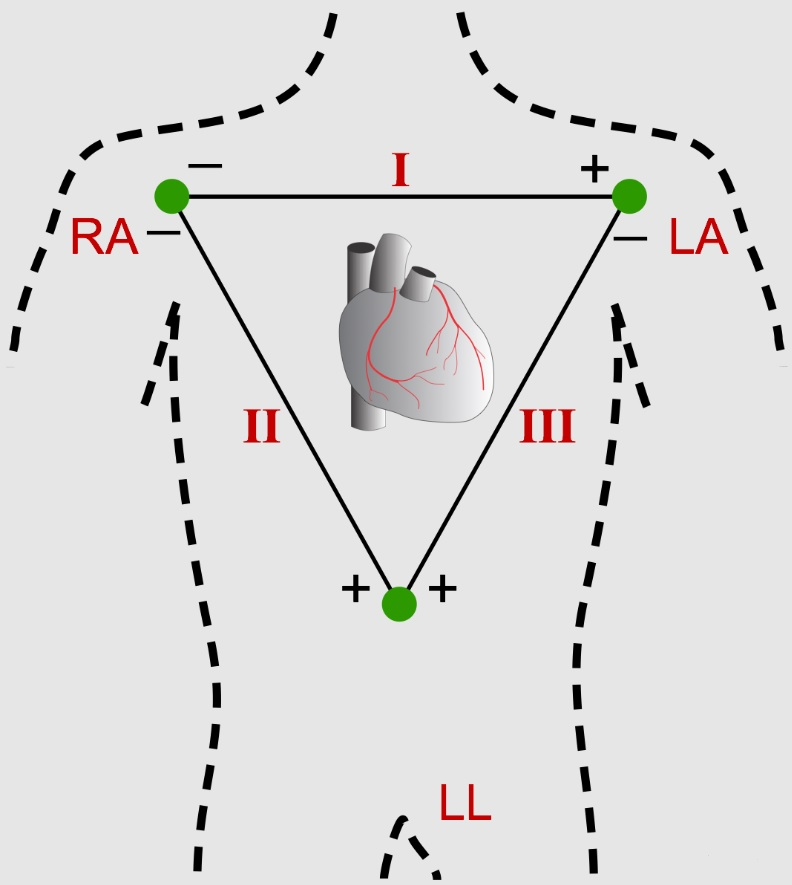
\includegraphics[width=0.5\textwidth]{images/einthoven traingle}
	\caption{Einthoven's Triangle~\cite{cvphysiology}}
	\label{fig:einthoven_triangle}
\end{figure}

\noindent This setup involves placing electrodes on the left arm (LA), right arm (RA), and left leg (LL). The potential difference measured across each lead is derived from the relative placement of these electrodes according to the Einthoven Triangle:\\
\begin{itemize}
	\item \textbf{Lead I:} Measures the potential difference between the left arm (LA) and right arm (RA).
	\item \textbf{Lead II:} Measures the potential difference between the left leg (LL) and right arm (RA).
	\item \textbf{Lead III:} Measures the potential difference between the left leg (LL) and left arm (LA).
\end{itemize}

\noindent Three-lead ECG systems are commonly utilized in Mobile Cardiac Telemetry (MCT) for continuous monitoring, especially useful for detecting cardiac artifacts\cite[chap. 1, p. 4]{conover2002}\cite{tsang2013}.\\

\subsection{12-Lead ECG Systems}
\vspace{1em}
\noindent Building on Einthoven's foundational work, Goldberger expanded the diagnostic capabilities of ECG by introducing augmented leads known as aVR, aVL, and aVF. These leads were designed to provide additional views of cardiac activity to address gaps in the data provided by the original three leads. Goldberger employed the "Wilson central terminal" (WCT), a reference point established by connecting the three limb electrodes (right arm, left arm, and left leg). The electric potentials for the augmented leads relative to the WCT are specified the below equations-\cite{wagner2013, malminen1995}:

\begin{equation}
	aVF = LL - 0.5 \times (RA + LA)
\end{equation}
\begin{equation}
	aVL = LA - 0.5 \times (RA + LL)
\end{equation}
\begin{equation}
	aVR = RA - 0.5 \times (LA + LL)
\end{equation}

\noindent Figure~\ref{fig:leads} below illustrates the configurations of limb leads (I-III) and augmented leads (aVR, aVL, aVF), which together provide comprehensive information about the frontal plane of the heart.

\begin{figure}[H]
	\centering
	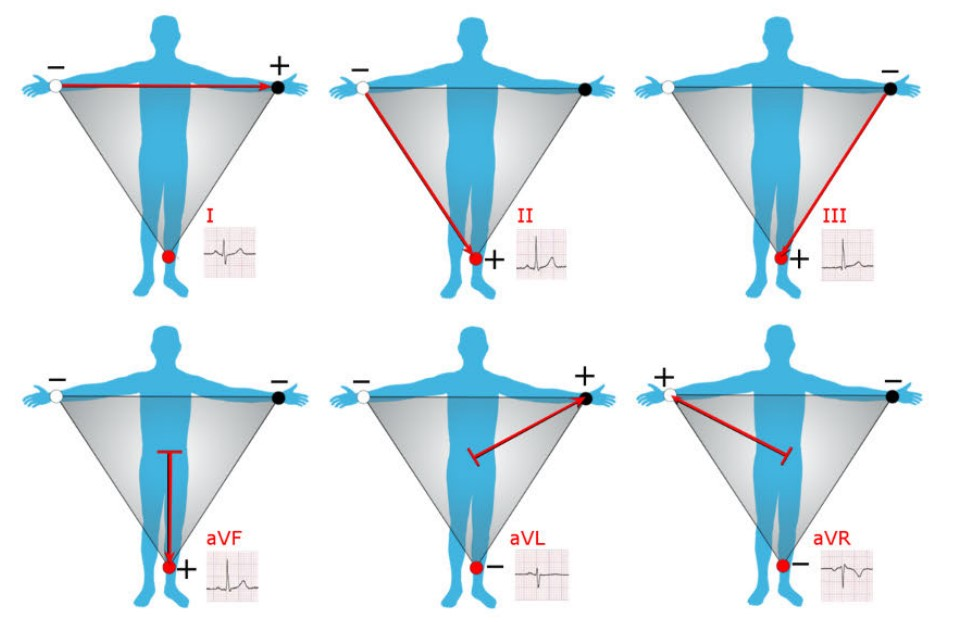
\includegraphics[width=0.7\textwidth]{images/3lead and augumented lead}
	\caption{Illustration of Limb Leads(Top) and Augmented Leads(Bottom) \cite{wasimuddin2020}}
	\label{fig:leads}
\end{figure}

\noindent To further enhance the understanding of the heart’s transverse plane, Wilson introduced six precordial leads (V1 to V6). In this setup, the positive electrode is connected to a specific precordial site, while the negative electrode is linked to the WCT\cite{hall2015, malminen1995}. The potential difference between these electrodes defines the voltage for each precordial lead given as-

\begin{equation}
	VL = V'L - \text{WCT}
\end{equation}

Here, \( V'L \) represents the voltage recorded at the L\textsuperscript{th} precordial electrode, and WCT is calculated as:

\begin{equation}
	\text{WCT} = \frac{1}{3} \times (RA + LA + LL)
\end{equation}

\noindent The combination of limb leads, augmented leads, and precordial leads comprises the 12-lead ECG system, which utilizes nine electrodes (three for the limbs and six for the precordial) to generate twelve distinct waveforms corresponding to each lead.Additionally, a Right lead electrode is used for reference as discussed in \ref{RLD}. This system is depicted in Figure \ref{fig:12_lead_ecg}.
\begin{figure}[H]
	\centering
	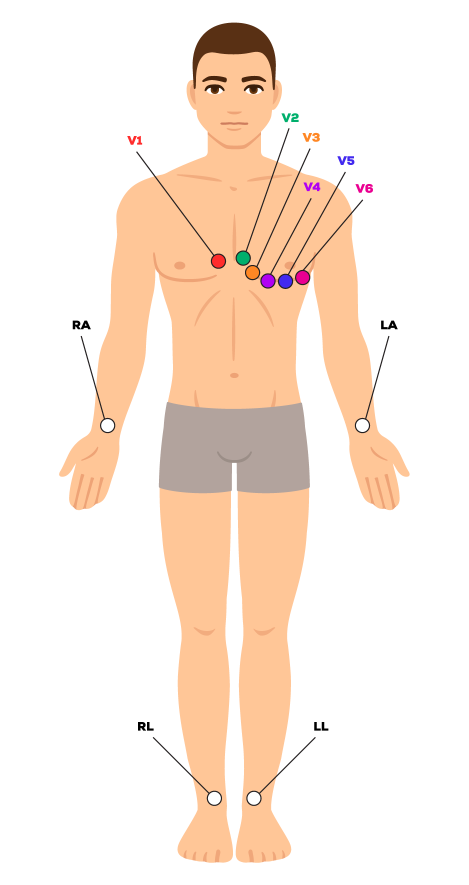
\includegraphics[width=0.3\textwidth]{images/12lead placement}
	\caption{12-Lead ECG Electrode Configuration \cite{cardiacdirect_ecg}}
	\label{fig:12_lead_ecg}
\end{figure}

\noindent The 12-lead ECG is considered the gold standard for monitoring all types of cardiac activities. Despite its comprehensive capabilities, the complex arrangement of electrodes makes the 12-lead ECG less suitable for daily, long-term monitoring. On the other hand, the three-lead system, with a specificity of 98.7\% for detecting atrial fibrillation (AF), is often preferred for this purpose due to its simpler setup and effectiveness in diagnosing AF \cite{kristensen2016}.

\subsection{Single-Lead ECG Systems}
\vspace{1em}
\noindent Single-lead ECG systems have gained increasing relevance in recent years. They utilize just one of the leads from the Einthoven triangle, making them particularly suited for prolonged continuous monitoring of ECG data, typically over 24 to 48 hours. Their simplicity and ease of use make them ideal for outpatient settings and home monitoring.\\

\noindent One significant challenge in single-lead ECG systems is the necessity for a specialized front-end ECG acquisition stage. This requirement stems from the absence of a reference electrode, which is usually provided by the driven right leg (DRL) circuit \ref{RLD}. The front-end design must compensate for this by ensuring a high Common Mode Rejection Ratio (CMRR) \cite{babusiak2015}. This design enhances the ability of the differential amplifier to discriminate between the desired biological signals and unwanted noise, thereby improving the quality and reliability of the ECG data captured.\\

\noindent In this thesis, we explore such a front-end circuit, focusing on its design and implementation within our ECG detection system. This examination will provide insights into the technical adaptations needed to optimize single-lead ECG systems for effective cardiac monitoring.\\


\section{Challenges in ECG Monitoring}
\vspace{1em}
\noindent Accurate diagnosis from ECG readings relies heavily on signal quality. The clinically useful information in an ECG waveform is typically found within the frequency range of 0.05 to 100 Hz and has a dynamic range of 1 to 10 mV \cite{Velayudhan2016NoiseAA}. High-quality signals are crucial for the accuracy and reliability of ECG diagnoses. However, various types of noise can interfere with signal acquisition, merging with the ECG signal and potentially hindering accurate diagnosis.\\

\noindent Noise in ECG signals generally falls into two categories: high-frequency and low-frequency noises. High-frequency noises like Electromyogram noise, Additive white noise, and power line Interference while Low-frequency noises include baseline wandering and motion artifacts \cite{Velayudhan2016NoiseAA}.\\

\subsection{Types of Noise in ECG Signals}\label{noises}
\vspace{1em}
\subsubsection{Power Line Interference}
\vspace{1em}
\noindent Power line interference is a type of common-mode noise affecting ECG signals due to electromagnetic fields generated by power lines. This interference typically manifests as a 50/60 Hz sinusoidal wave, often accompanied by harmonics, resulting from AC fields produced by looped wires, poor grounding, or bad contacts. Suppressing this interference is crucial as it can obscure the low-amplitude signals of the ECG, such as the P, Q, S, and T waves \cite{Velayudhan2016NoiseAA,Kher2019SignalPT}.

\begin{figure}[h]
	\centering
	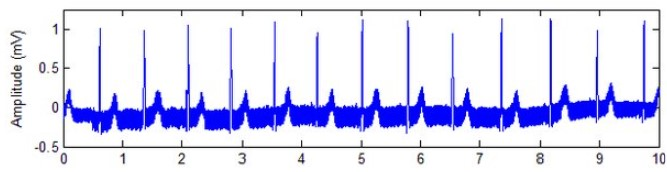
\includegraphics[width=0.8\textwidth]{images/powerline noise}
	\caption{Power Line Interference in ECG \cite{Maggio2012Quantification}}
	\label{fig:power_line_interference}
\end{figure}

\subsubsection{Baseline Wander}
\vspace{1em}
\noindent Baseline wander, or drift, occurs when the baseline of the ECG signal shifts vertically instead of remaining straight. This noise is predominantly caused by patient movement and respiration, typically at frequencies below 1 Hz \cite{Kher2019SignalPT}.

\begin{figure}[h]
	\centering
	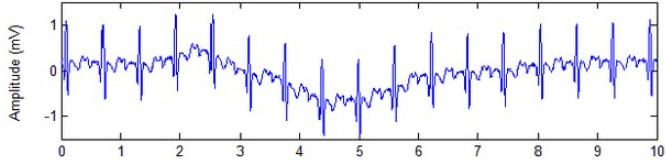
\includegraphics[width=0.8\textwidth]{images/baseline wander}
	\caption{Baseline Wander in ECG \cite{Maggio2012Quantification}}
	\label{fig:baseline_wander}
\end{figure}

\subsubsection{Electromyogram (EMG) Noise}
\vspace{1em}
\noindent Electromyogram noise is high-frequency interference arising from muscle activity during the recording of ECG, which can reach frequencies up to 10 kHz \cite{Velayudhan2016NoiseAA,Kher2019SignalPT}. This type of noise interferes with the ECG signal.

\begin{figure}[h]
	\centering
	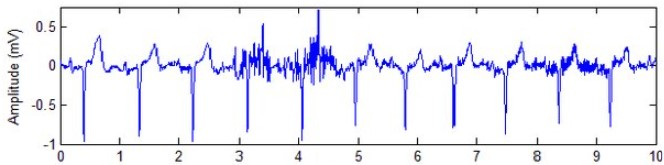
\includegraphics[width=0.8\textwidth]{images/emg_noise}
	\caption{EMG Noise in ECG \cite{Maggio2012Quantification}}
	\label{fig:emg_noise}
\end{figure}

\subsubsection{Motion Artifacts}
\vspace{1em}
\noindent Motion artifacts, similar to baseline wander, significantly affect ECG signals. They can distort the entire PQRST complex due to changes in skin impedance caused by skin stretching near the electrodes. These artifacts typically occur in the 1 to 10 Hz frequency range~\cite{Kher2019SignalPT} and can be seen in Figure \ref{fig:motion_artifacts}.

\begin{figure}[h]
	\centering
	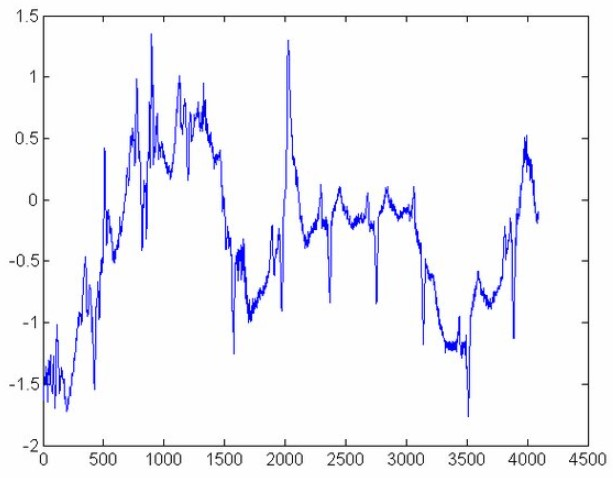
\includegraphics[width=0.6\textwidth]{images/motionArtifacts}
	\caption{Motion Artifacts in ECG \cite{Kher2019SignalPT}}
	\label{fig:motion_artifacts}
\end{figure}

\noindent Understanding and addressing these noise types is essential for improving ECG signal quality and ensuring accurate cardiac monitoring and diagnosis.\\


\subsection{Strategies for Noise Reduction}
\vspace{1em}
\noindent Reducing noise in ECG signals involves distinguishing and removing unwanted interference while preserving the original signal's integrity. Effective noise reduction can be achieved primarily through two methods: utilizing a front-end circuit to diminish common mode noise before it reaches the differential stage, and employing various filtering techniques to isolate the essential frequency components of the ECG signal. We will explore a notable method for common mode noise reduction and some filtering techniques commonly referenced in literature.\\

\subsubsection{Driven Right Leg (RLD)}\label{RLD}
\vspace{1em}
\noindent The RLD technique enhances ECG systems by mitigating common mode noise using an additional electrode attached to the right leg. This electrode, while not directly involved in diagnostic measurements, serves as a reference point for the ECG system and redirects common mode noise back to the body. Originally introduced by Winter and Webster, the RLD method typically employs a differential amplifier as a front-end circuit to further reduce common mode noise and enhance signal sensitivity \cite{Winter1983Driven}.\\

\noindent The RLD utilizes the "Wilson central terminal technique," where a node averaging all electrode potentials is created. This node effectively nullifies differential mode signals and provides a low-resistance pathway for common mode signals. As illustrated in Figure \ref{fig:rld_circuit}, common mode signals ($I_3$), facilitated by averaging resistors ($R_a$), are inverted and re-introduced to the body through the right leg electrode $RL$, enhancing overall ECG signal clarity.

\begin{figure}[htbp]
	\centering
	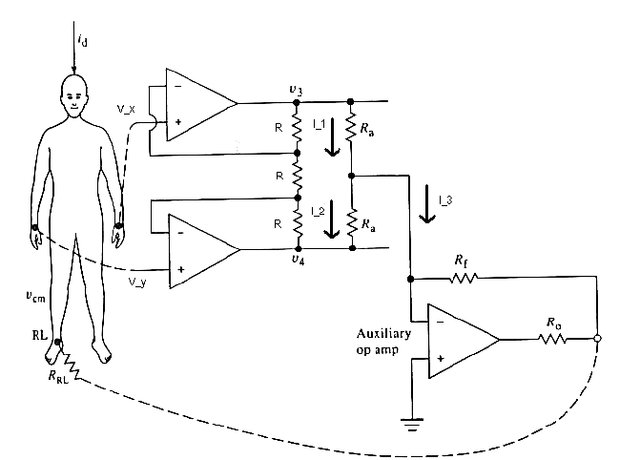
\includegraphics[width=0.7\textwidth]{images/driven right leg}
	\caption{Driven Right Leg Circuit Schematic \cite{Saha2018Design}}
	\label{fig:rld_circuit}
\end{figure}

\subsubsection{Filtering Techniques}
\vspace{1em}
\noindent Various filtering techniques are discussed extensively in the literature to address different types of noise \cite{Luo2010Review}. Filtering techniques are normally classified into two types: digital filtering, which is done at the backend after extracting the raw noisy data, and analog filtering, which is done during the extraction of the ECG signal.

\begin{itemize}
	\item \textbf{Notch Filters:} These are used specifically to eliminate power line interference, typically at 50/60 Hz.
	\item \textbf{Low-Pass Filters:} These filters remove high-frequency noise above 150 Hz, which is beyond the range of typical ECG signals.
	\item \textbf{High-Pass Filters:} Employed to eliminate low-frequency noises such as baseline drift and motion artifacts.
	\item \textbf{Antialiasing Filters:} These are crucial just before the analog-to-digital conversion process, particularly when the sampling frequency does not meet the Nyquist criterion. This helps prevent aliasing from corrupting the digital ECG signal.
\end{itemize}

\noindent The selection of a specific filter depends on the characteristics of the ECG signal needed for accurate diagnosis and the type of noise interference present in the signal environment.\\

\section{Architectures for ECG Data Acquisition}
\vspace{1em}
\noindent Wearable health devices are increasingly favored for their ability to monitor heart activity continuously, minimize discomfort, and interfere with daily activities. These devices, typically battery-powered, support both real-time and offline data monitoring. Understanding the architecture of these systems, as well as identifying areas for improvement, is crucial for advancing their effectiveness.

\subsection{Remote and Offline Monitoring Architectures}
\vspace{1em}
\noindent According to various literature reviews, the architecture depicted in Figure \ref{fig:wbna_architecture} represents a generic setup for wearable continuous monitoring utilized in both researched prototypes and commercial products. This system architecture is often referred to as a “Wireless Body Area Network” (WBAN).

\begin{figure}[htbp]
	\centering
	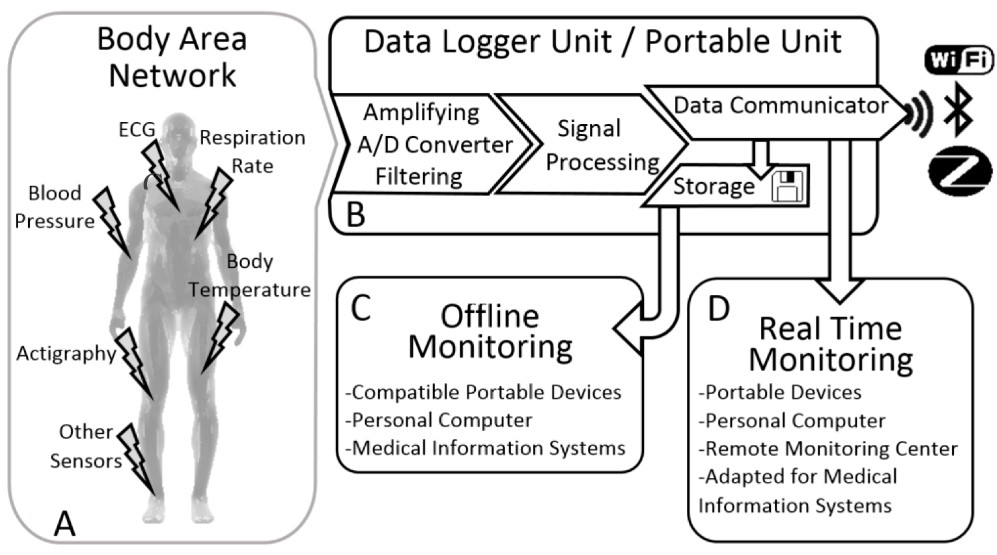
\includegraphics[width=0.7\textwidth]{images/remote architecture}
	\caption{WBAN Architecture~\cite{Dias2018Wearable}}
	\label{fig:wbna_architecture}
\end{figure}

\noindent\textbf{Body Area Network (BAN)}

\noindent A BAN consists of interconnected sensor nodes, each dedicated to monitoring specific body parameters. Each node is equipped with a sensor system, a controller, and a memory unit. Data, whether raw or filtered, is transmitted from the sensor nodes to a central data logger unit for further processing. Connection to a central portable unit via wired or wireless means centralizes and synchronizes the data, crucial for effective continuous monitoring. In the case of continuous monitoring, only a single node is connected directly to the Data logger unit for processing, storing, and transmitting \cite{Dias2018Wearable, Pantelopoulos2010Survey}.\\

\noindent\textbf{Data Logger/Portable Unit}

\noindent This component logs data from various sensor nodes. It receives analog signals, converts them to digital via an A/D converter, and processes the data to extract additional information, such as heart rate from ECG, using measurements like RR peak distances. Data can be utilized for immediate real-time monitoring or stored for later analysis \cite{Dias2018Wearable}.\\

\noindent\textbf{Real-Time Monitoring}

\noindent Advancements in AI allow data from the portable unit to be sent to remote servers where various machine learning algorithms classify different abnormalities in real time. Transmission utilizes wireless protocols such as Bluetooth, BLE, Zigbee, GSM, and WiFi \cite{Dias2018Wearable, Shaown2019IoT}.\\

\noindent\textbf{Offline Monitoring}

\noindent Data can also be archived on portable storage devices such as micro SD cards or USB drives for future analysis by medical professionals or for personal health records \cite{Dias2018Wearable}.\\

\noindent\textbf{Challenges}

\noindent Despite the benefits, several challenges persist in this architecture as\cite{Muhoza2023Power, Lim2010Security}-:

\begin{itemize}
	\item \textbf{Power Consumption:} Continuous data transmission, especially using WiFi or BLE, can be energy-intensive.
	\item \textbf{Latency:} High data traffic can lead to congestion and increased latency.
	\item \textbf{Security:} Ensuring data privacy and security remains a concern. Encrypting data before transmission requires considerable computational power, which may not be feasible for battery-operated devices.
\end{itemize}


\subsection{Edge-Based Monitoring Architectures Using AI}
\vspace{1em}
\subsubsection{Edge AI-related Work}

\noindent Edge AI involves integrating artificial intelligence algorithms directly into microcontroller-based devices, contrasting with remote AI, which relies on cloud or remote servers for computation. Research indicates that Edge AI significantly reduces energy consumption and latency compared to cloud-based AI solutions \cite{Muhoza2023, Himeur2024, Vita2020}. A notable study \cite{Muhoza2023} employed an ARM Cortex-based microcontroller to run a DCNN model that predicted human activity from accelerometer data, highlighting the efficiency of Edge AI through two scenarios:\\

\noindent\textbf{Scenario 1 (Remote AI):}

\noindent In this scenario, as soon as the data is acquired from the accelerometer sensor, it is directly transmitted to a remote server using BLE communication for AI computation as shown in Figure \ref{fig:remote_ai}. In this scenario, there is no intervention of the AI algorithm used at the sensor node \cite{Muhoza2023}.

\begin{figure}[h]
	\centering
	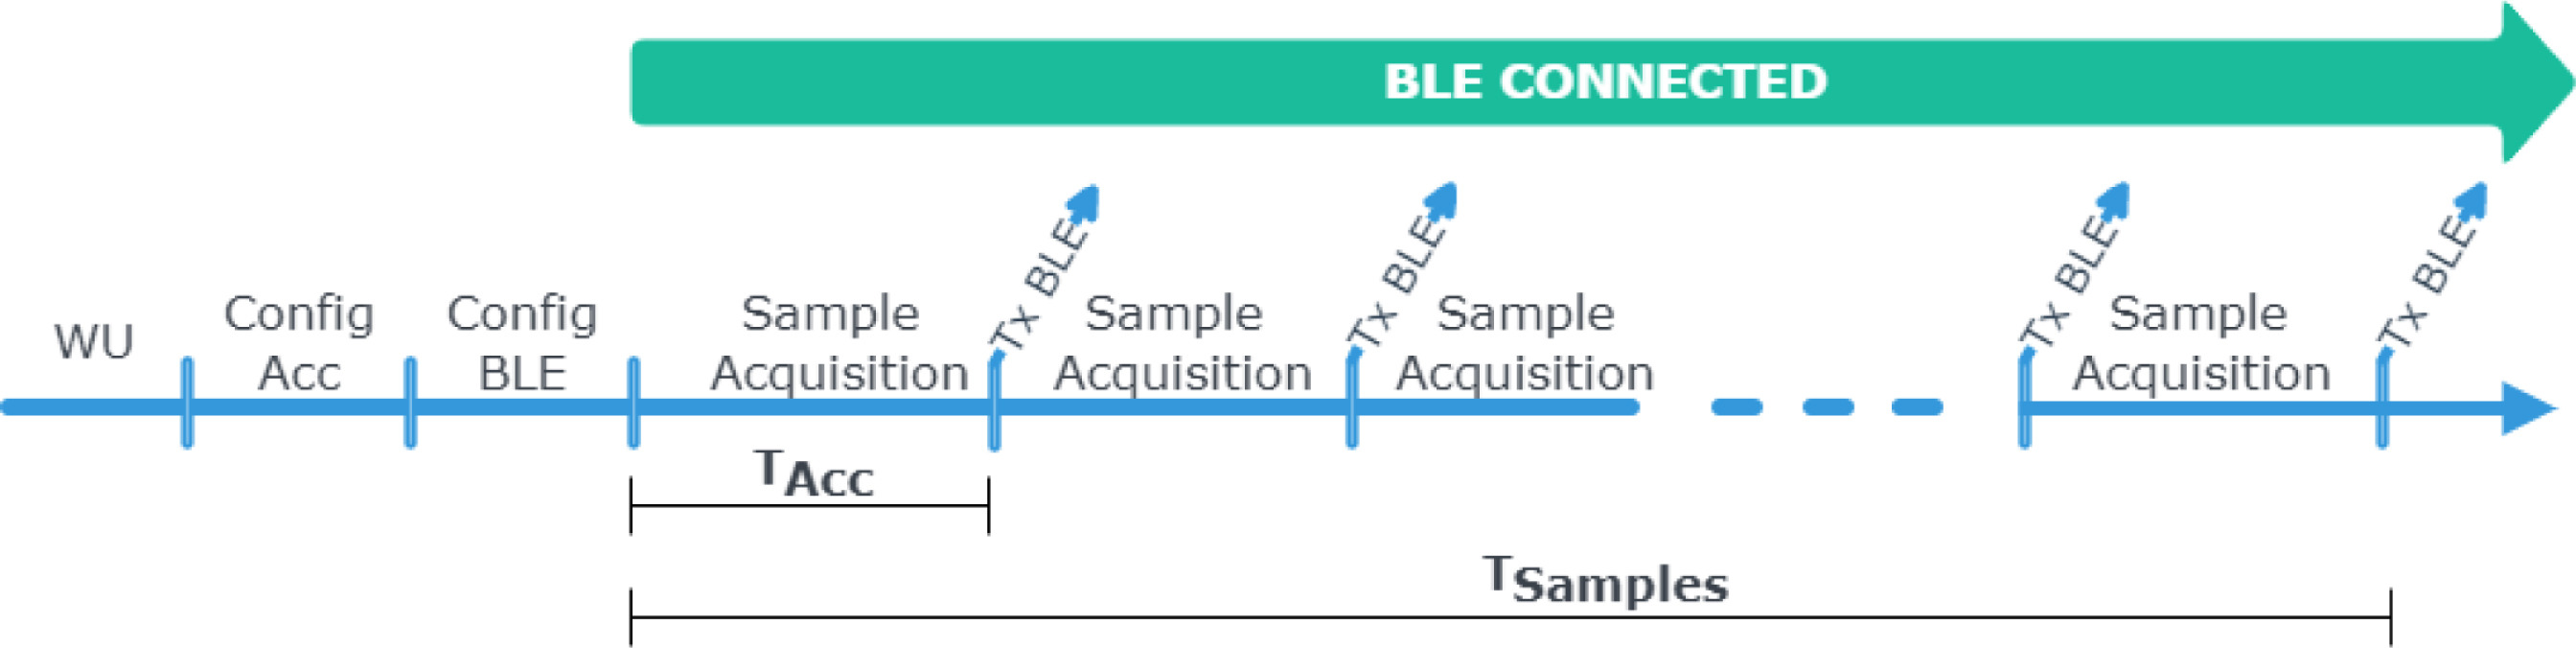
\includegraphics[width=0.8\textwidth]{images/senerio1}
	\caption{Remote AI Data Flow~\cite{Muhoza2023}}
	\label{fig:remote_ai}
\end{figure}

\noindent\textbf{Scenario 2 (Edge AI):}

\noindent In this scenario, the DCNN model running on an edge microcontroller processes data locally every 100 samples. It achieves an F1 score of 98.3\% in classifying human activities. DCNN results classification is buffered locally and only transmitted when the buffer is full, significantly reducing BLE usage and power consumption, as BLE is only active and connected when the buffer is ready to transmit. The DCNN model used consisted of two successive 1D convolution layers, a pooling layer, two fully connected layers, and a softmax layer for activity prediction \cite{Muhoza2023}.

\begin{figure}[h]
	\centering
	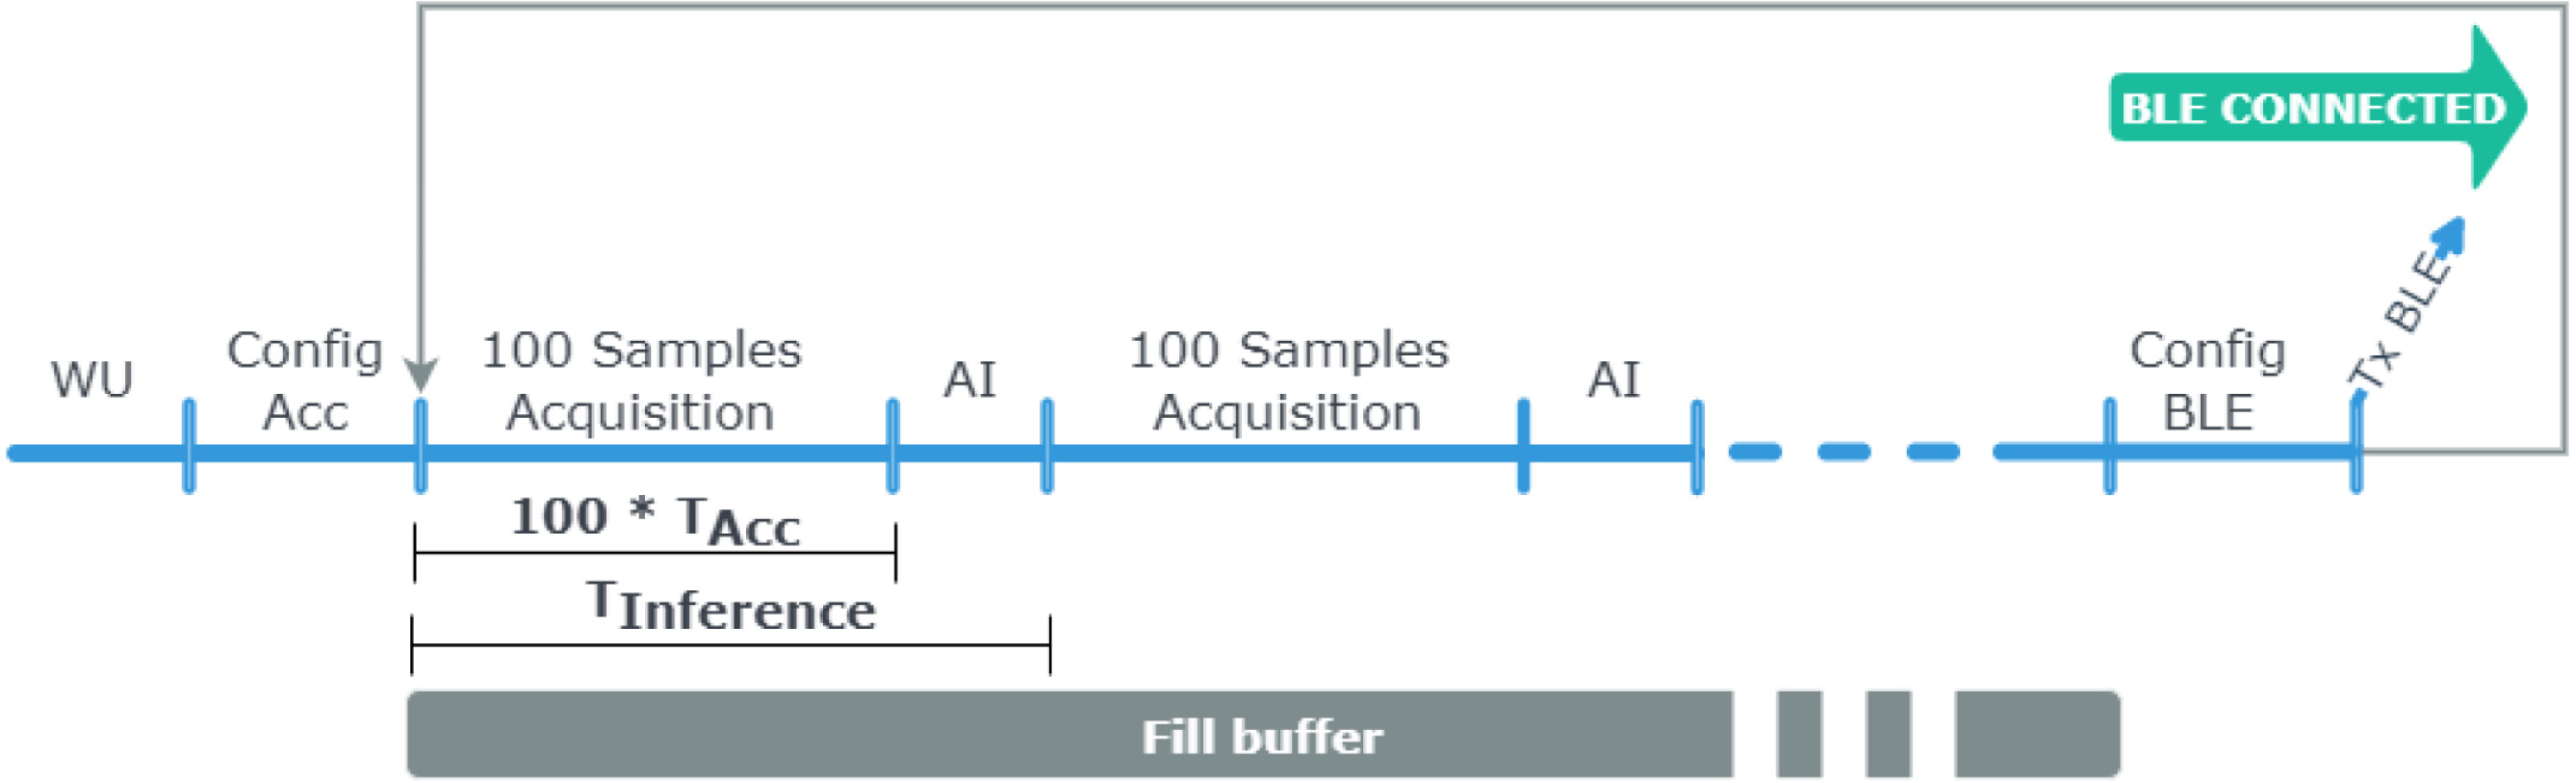
\includegraphics[width=0.8\textwidth]{images/SENERIO2}
	\caption{Edge AI Data Flow~\cite{Muhoza2023}}
	\label{fig:edge_ai}
\end{figure}

\noindent Comparative analysis showed that Scenario 2 saved up to 20\% battery life over an hour compared to Scenario 1, while also minimizing Bluetooth congestion, which is notable since the BLE module consumes considerable power during data transmission \cite{Muhoza2023}.

\begin{figure}[h]
	\centering
	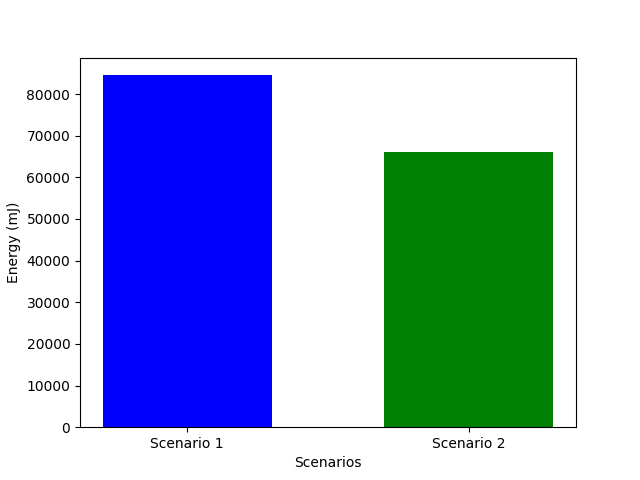
\includegraphics[width=0.7\textwidth]{images/senerio comparision}
	\caption{Battery Usage Comparison (redrawn from \cite{Muhoza2023})}
	\label{fig:battery_usage}
\end{figure}

\subsubsection{Edge AI-based Architecture}
\vspace{1em}
\noindent A survey of literature on Edge AI underscores the need for integrating AI processing within wearable monitoring systems to enhance remote monitoring architectures. By incorporating an Edge AI element just before data transmission to a remote server, a new architecture emerges, significantly optimizing power and data latency \cite{Muhoza2023, Shaik2023, Mujawar2020, Ashfaq2022}. This architecture utilizes DNN models to process digital data post-A/D conversion, dramatically enhancing battery efficiency and reducing latency.

\begin{figure}[h]
	\centering
	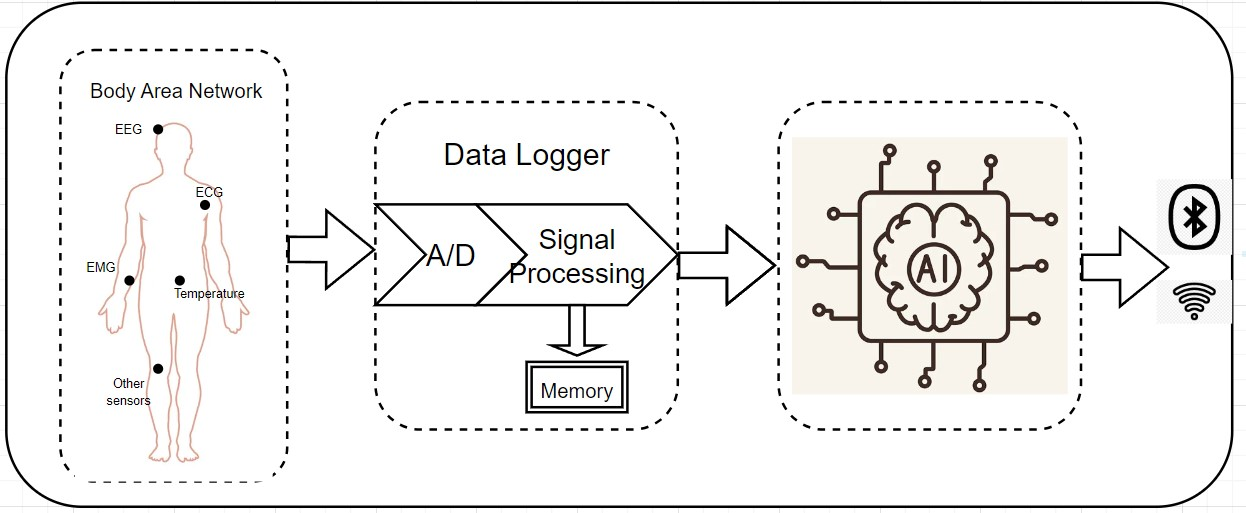
\includegraphics[width=0.8\textwidth]{images/ai on edge arch}
	\caption{Edge AI-Based Architecture (redrawn from \cite{Muhoza2023, Shaik2023, Mujawar2020, Ashfaq2022})}
	\label{fig:edge_ai_based_architecture}
\end{figure}

\noindent This thesis will explore this Edge AI-based architecture, comparing its performance with traditional remote and offline monitoring setups in terms of energy efficiency and effectiveness in detecting atrial fibrillation (AF) in ECG signals.\\

\subsubsection{Edge AI-based DNN Accelerators}
\vspace{1em}
\noindent Recent advancements in deep neural networks (DNN) have led to models that more closely mimic real-world sensory systems, though they have become computationally and memory-intensive. Deploying such models on microcontrollers often results in systems that are unsuitable for battery-powered devices due to high energy demands.\\

\noindent To mitigate energy and memory inefficiency, novel hardware architectures have been developed specifically for handling DNN-based workloads \cite{Moss2023, Reuther2021}. These architectures typically feature on-chip memory to minimize power consumption and latency associated with data transfer from off-chip memory. They also include large computational arrays for performing operations such as addition and matrix multiplication, and dedicated data flow paths between computational cores to enhance data reuse. Most operate with low-precision computing, like 8-bit operations, to balance performance with energy efficiency. Figure \ref{fig:dnn_hardware_comparison} illustrates a comparison of power usage against GOPs (Giga Operations per second) for various hardware architectures designed by different companies \cite{Moss2023}.\\

\begin{figure}[h]
	\centering
	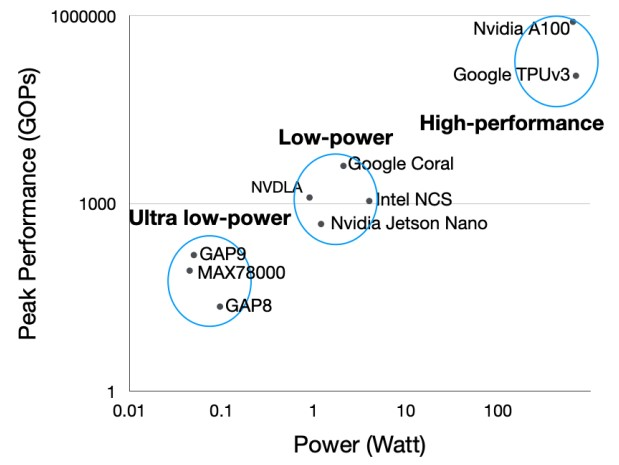
\includegraphics[width=0.6\textwidth]{images/power vs gops}
	\caption{Comparison of Power Consumption and Computational Capacity in DNN Hardware Architectures~\cite{Moss2023}}
	\label{fig:dnn_hardware_comparison}
\end{figure}

\noindent Among these, ultra-low power hardware accelerators are particularly suited for battery-operated biosensing devices. The Max78000, for example, is a system-on-chip that executes neural networks with ultra-low power consumption. It combines a dual-core microcontroller (ARM Cortex-M4 and a RISC-V co-processor) with a dedicated CNN hardware accelerator, capable of supporting deep CNN networks up to 64 layers with 64 parallel processors. This allows for both 1D and 2D convolution processing. The CNN engine includes its own weight memory of 441KB and supports up to 8-bit weight precision \cite{MAX78000-datasheet}. Figure \ref{fig:max78000_hardware} shows the hardware architecture of the Max78000.

\begin{figure}[h]
	\centering
	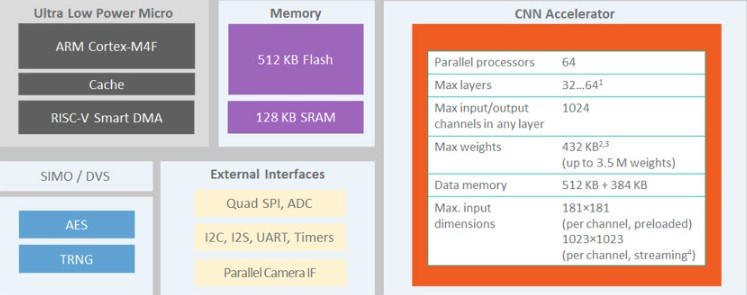
\includegraphics[width=0.8\textwidth]{images/max78000arch}
	\caption{MAX78000 Hardware Architecture~\cite{analog-devices-max78000-app-note}}
	\label{fig:max78000_hardware}
\end{figure}

\noindent This thesis will explore the integration of the MAX78000-based feather board with an ECG circuit board to classify heart rate abnormalities and related diseases.\\

\section{Security in Medical Sensing}
\vspace{1em}
\noindent As medical sensing devices increasingly integrate with the Internet of Things (IoT), securing sensitive health data becomes paramount. These devices frequently transmit data to remote servers for analysis and storage, making them potential targets for cybersecurity threats. Breaches can compromise patient privacy and lead to serious health risks, such as incorrect diagnoses or inappropriate medical interventions \cite{Paul2023, Abdunabi2023}.

\begin{itemize}
	\item \textbf{Vulnerability of Medical Data:} The integration of IoT in medical devices exposes them to various security vulnerabilities, particularly at the point of data transmission. Devices using wireless communication technologies like Bluetooth Low Energy (BLE) or Zigbee are especially susceptible to eavesdropping and interference \cite{Paul2023, Bresson2004}. The potential for data interception or manipulation can lead to catastrophic outcomes, including the administration of incorrect medical treatments.

	\item \textbf{Strategies for Enhancing Security:} Literature on the topic suggests multiple approaches to protect against these vulnerabilities. The implementation of strong encryption protocols is a primary method for securing data transmitted between IoT devices and remote servers. Encrypting data ensures that even if data interception occurs, the information remains unintelligible without the proper decryption keys \cite{Paul2023, Bresson2004}.

	\item \textbf{Security Implementation Challenges:} Encryption enhances data security but also adds extra computational overhead and power consumption. Implementing a security node just before sending data to the server involves substantial energy-intensive operations.

	\item \textbf{Edge AI for Enhanced Security:} Utilizing edge AI architecture can significantly reduce the amount of data needing transmission by processing data directly on the device. This approach limits the exposure of raw data to potential security threats. For instance, devices can analyze and process ECG data locally to determine the presence of atrial fibrillation and only transmit the essential summarized data or alerts to healthcare providers. This reduces the bandwidth needed for data transmission, decreases the risk of data interception, and conserves energy \cite{Paul2023}.
\end{itemize}

\noindent This thesis explores the use of the Infineon OPTIGA™ Trust M, a security solution integrated into the edge AI architecture. This module provides robust security by handling cryptographic operations directly on the chip, thus safeguarding data integrity and authenticity from the point of capture to storage and analysis. The integration of such security elements demonstrates how advanced hardware can be leveraged to enhance data protection in medical IoT devices without excessive power consumption \cite{infineon-optiga-trust}.\\

	
	% !TeX root = ../thesis.tex

\chapter{System Design and Development}
\label{chap:system_design_and_development}

This chapter delineates the detailed methodologies employed in designing, developing, and validating the ECG monitoring system. It is divided into two main sections: ECG Circuit Board Design and Development, and Integration of the Max78000 Feather Board, with each aspect discussed in detail.

\section{ECG Circuit Board Design and Development}
\vspace{1em}
\subsection{Overview of ECG Signal Acquisition}
\vspace{1em}
Building on the insights from Chapter 2, this thesis involves developing a single-lead ECG circuit designed to accurately detect R peaks and classify heart rate abnormalities. Given the typical ECG signal range of 1 to 5 mV, it is essential to integrate a high-gain stage to amplify the signal adequately. Additionally, effective filtering techniques are crucial to eliminate low and high-frequency noises, including the common 50Hz power noise. The design also incorporates a system for reducing common mode noise.

\subsubsection{Specification}
\vspace{1em}
The objective was to design a single-lead ECG circuit optimized for continuous monitoring using a battery-powered system. The specifications were determined as follows:
\begin{itemize}
	\item Total gain of 1000
	\item High pass filter with a cutoff frequency of 6 Hz
	\item Low pass filter with a cutoff frequency of 20 Hz
	\item Common mode noise reduction circuit
	\item DC Reference circuit
	\item Protection circuit for EMI and overvoltage
	\item External 3.7V battery power system
\end{itemize}

\subsubsection{Block Diagram}
\vspace{1em}
Based on the above specifications, a block diagram was developed to outline the ECG signal acquisition process, as depicted in Figure \ref{fig:ecg_block_diagram}. The diagram illustrates the sequential arrangement of various stages:

\begin{figure}[H]
	\centering
	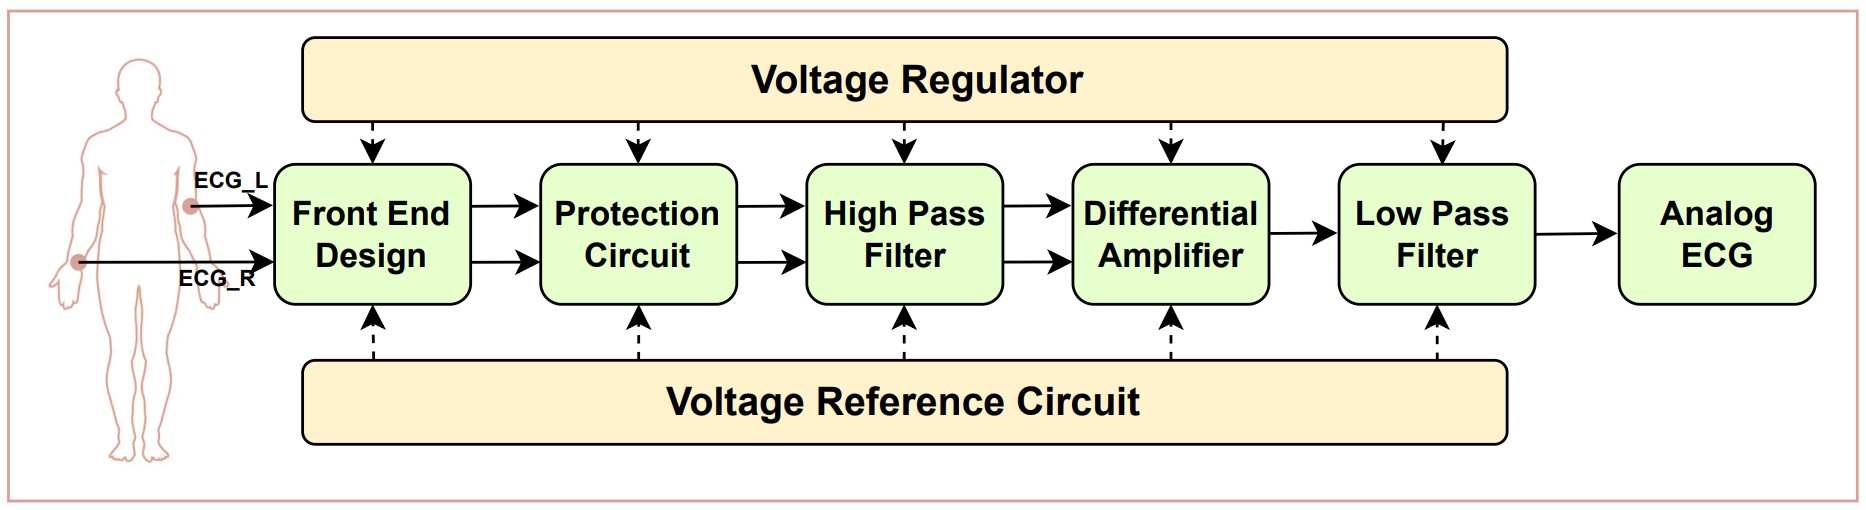
\includegraphics[width=0.8\textwidth]{images/block_diagram_ecg}
	\caption{Block Diagram of ECG Signal Acquisition}
	\label{fig:ecg_block_diagram}
\end{figure}

\begin{itemize}
	\item \textbf{Front-End Circuit:} Captures differential signals while minimizing common-mode signals and providing a DC reference.
	\item \textbf{Protection Circuit:} Shields the device from overvoltage and EMI at the input stage.
	\item \textbf{First Filter Stage (High-Pass Filter):} Reduces DC drift from input lines.
	\item \textbf{Differential Amplifier Stage:} Amplifies the voltage difference between the two electrodes to produce an amplified ECG signal.
	\item \textbf{Low-Pass Filter:} Removes high-frequency noise while further amplifying the signal.
	\item \textbf{Analog-to-Digital Converter (A/D):} Digitizes the amplified signal in the microcontroller for subsequent processing.
	\item \textbf{Power Circuit:} Supplies a regulated 3.3V to the analog circuit and an additional voltage reference of Vcc/2.
\end{itemize}



\subsection{Detailed Design Process}
\vspace{1em}
This section elaborates on the detailed design process for each component illustrated in the block diagram. The entire design operates on a 3.7V lithium-ion battery, regulated to a constant 3.3V using a linear regulator.

\subsubsection{Electrodes}
\vspace{1em}
To measure and record the heart's electrical potential, an interface between the body and the electronic measuring apparatus is necessary. This interface is provided by conductive pads known as electrodes, as shown in Figure \ref{fig:electrodes}, which are attached to the skin to enable the recording of heart electrical signals \cite{webster_medical_2020}. While electrodes can be invasive or noninvasive, this project utilizes noninvasive electrodes.\\

\noindent A commonly used type of noninvasive electrode is the Ag/AgCl electrode, a non-polarized variant. It features a metal stud at the center covered with Ag wire, surrounded by an AgCl layer. Between the electrode and the human skin, an electrolyte solution or gel is applied to facilitate current flow, which in the human body is ion-based. This electrode-electrolyte interface induces a chemical reaction, converting ion current into electron current. When Ag comes into contact with the electrolyte, it oxidizes, forming Ag\(^+\) ions and electrons (e\(^-\)). Simultaneously, AgCl reduces to Ag\(^+\) and Cl\(^-\) ions, shedding electrons (e\(^-\)). This ion distribution disparity creates a potential difference across the electrode-electrolyte interface, known as the half-cell potential \cite{lee_kruse_2020}. Figure \ref{fig:skin_electrode_interface} below illustrates the skin-electrode interface in terms of an electrical circuit.

\begin{figure}[h]
	\centering
	\begin{subfigure}{0.4\textwidth}
		\centering
		\includestandalone{standalones/Circuits/electrode}
		\caption{Electrical Model of Skin-Electrode Interface \cite{lee_kruse_2020}}
		\label{fig:skin_electrode_interface}
	\end{subfigure} % <-- Corrected: Closing the subfigure environment here
	\hfill % <-- Added space between subfigures
	\begin{subfigure}{0.4\textwidth}
		\centering
		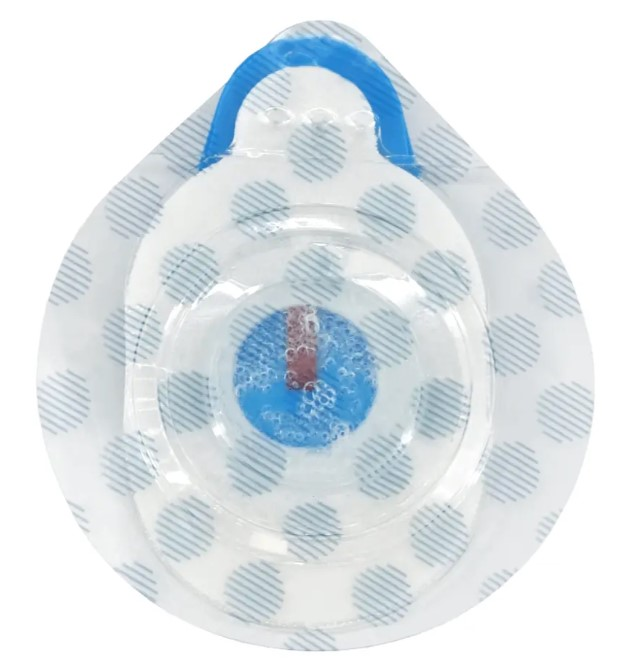
\includegraphics[width=0.8\textwidth]{images/electrodesample}
		\caption{Illustration of Electrodes\cite{blue_sensor_t00}}
		\label{fig:electrodes}
	\end{subfigure} % <-- Corrected: Closing the subfigure environment here
	\caption{Overview of Skin-Electrode Interface and Electrodes}
	\label{fig:electrodes_and_interface}
\end{figure}

		
		In this model:
		\begin{itemize}
			\item \(V_{ph}\) represents the half-cell potential developed due to the electrode-electrolyte interaction.
			\item \(R_p\) is the resistance between the electrode and skin during charge transfer.
			\item \(C_p\) indicates the electrical charge accumulated between the electrode and skin, with the electrolyte acting as the dielectric.
			\item \(R_s\) corresponds to the series resistance from the electrolyte gel, sweat, and skin tissue.
		\end{itemize}
		Standard values defined by IEC 60601 include \(R_d = 51\,k\Omega\) and \(C_d = 47\,nF\) \cite{Almeida_2021}. The impedance between the skin and electrode can vary significantly depending on the materials used and the quality of electrical contact. A high variance in impedance across electrode pairs can lead to common mode noise transforming into differential mode noise, which distorts the ECG waveform. For this thesis, we have chosen Ag/AgCl based non-polarized electrodes due to their low half-cell potential of approximately 220 mV. Figure \ref{fig:skin_electrode_interface} is also used in the SPICE simulation model to accurately represent the electrode's behavior in the circuit.


\subsubsection{Front-End Circuit Design}
\vspace{1em}
This thesis introduces a 2-electrode ECG acquisition system designed to obviate the need for a reference electrode, aiming to simplify the design complexity and reduce costs. A primary challenge in two-electrode systems is their susceptibility to common-mode noise, as they lack dedicated mechanisms for its mitigation, depending primarily on the common-mode rejection ratio (CMRR) of the differential amplifier.\\

\noindent To address the issues arising from the absence of a reference electrode, a front-end circuit configuration was adopted from the literature \cite{Dobrev_2008}. The primary objectives of this circuit are to establish a stable reference potential for each electrode and to alleviate the burden on the CMRR of the differential amplifier.\\

\noindent The front-end circuit was designed to fulfill several key functions:
\begin{itemize}
	\item High differential input impedance to prevent the ECG signal from loading.
	\item Sufficient low common mode input impedance to provide a low resistive path for common mode signal.
	\item Provide a reference voltage to each electrode.
\end{itemize}



\subsubsection*{A) Circuit Concept}

The conceptual design includes two identical inverting amplifiers, each constructed with resistors ($R_{1a} = R_{1b} = R_1$, $R_{2a} = R_{2b} = R_2$, $R_{3a} = R_{3b} = R_3$). These are arranged to form a positive feedback loop as depicted in Figure \ref{fig:front_end_circuit}. In this configuration, the electrodes for ECG acquisition, labeled as 'a' and 'b', are connected to the inverting inputs of the operational amplifiers (op-amps). The non-inverting inputs of the op-amps are connected to a reference voltage, set at $V_{cc}/2 = 1.65$V, suitable for single rail 0 to 3.3V op-amps.\\

\noindent The outputs from the op-amps feedback to the opposite electrodes through resistor $R_3$. For example, the signal from electrode 'a' passes through its corresponding op-amp and the output is connected to electrode 'b'. This setup ensures that electrode 'a' serves as a reference for electrode 'b', maintaining a consistent reference around 1.65V. Due to the circuit’s symmetry, the same principle is applied to the opposite electrode.\\

\noindent This arrangement of resistors $R_1$, $R_2$, and $R_3$ is critical as it ensures the circuit exhibits high differential mode impedance and adequate low common-mode impedance. These characteristics are essential for effectively addressing the challenges associated with a two-electrode ECG acquisition system, particularly in minimizing the impact of common-mode noise.

\begin{figure}[ht]
	\centering
	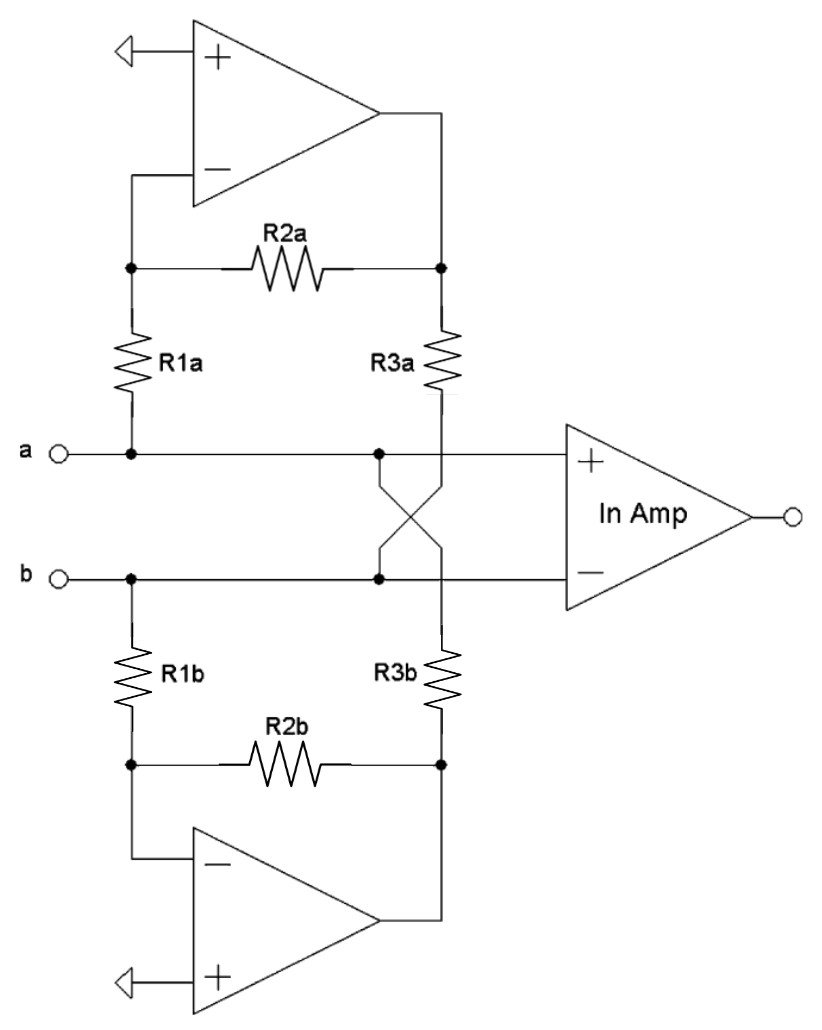
\includegraphics[width=0.5\textwidth]{images/frontend circuit}
	\caption{Conceptual Diagram of the Front-End Circuit (Redrawn from \cite{Dobrev_2008})}
	\label{fig:front_end_circuit}
\end{figure}


\subsubsection*{B) Circuit Analysis}
To determine the appropriate combination of resistors \(R_1\), \(R_2\), and \(R_3\)—ensuring very high differential impedance and sufficiently low common mode impedance—it is critical to perform a detailed analysis. This process helps in identifying the optimal resistance values for both differential and common mode resistance.

\begin{itemize}
\item \textbf{Differential Mode Analysis}


A simplified version of the front-end circuit with a differential voltage source is depicted in Figure \ref{fig:differential_mode}. In this configuration, both operational amplifiers with their feedback resistor \(R_2\) are represented by an ideal gain block. One end of resistor \(R_3\) is connected to half of the input differential voltage (\(V_d/2\)), and the other end is connected to the opposite half of the differential signal, facilitated by an inverting amplifier. To simplify analysis, assume the inverting amplifier's gain changes such that the gain coefficient \(G\) is defined as:
\begin{equation}
	G = \frac{R_2}{R_1}
	\label{eq:gain}
\end{equation}

The arrangement results in a simplified half-circuit equivalent of the front-end circuit for differential mode analysis, as shown in Figure\ref{fig:half_circuit_equivalent}.

\begin{figure}[h]
	\centering
	\begin{subfigure}{0.5\textwidth}
		\centering
		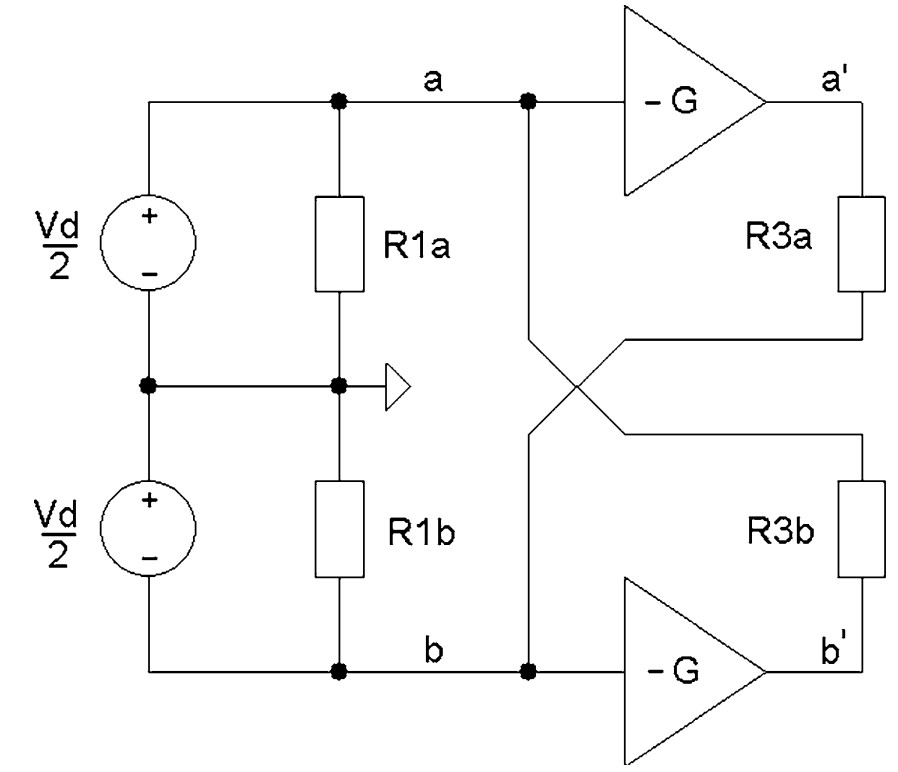
\includegraphics[width=0.8\textwidth]{images/diff_simplified}
		\caption{Simplified differential mode equivalent circuit}
		\label{fig:differential_mode}
	\end{subfigure}
	\hfill
	\begin{subfigure}{0.4\textwidth}
		\centering
		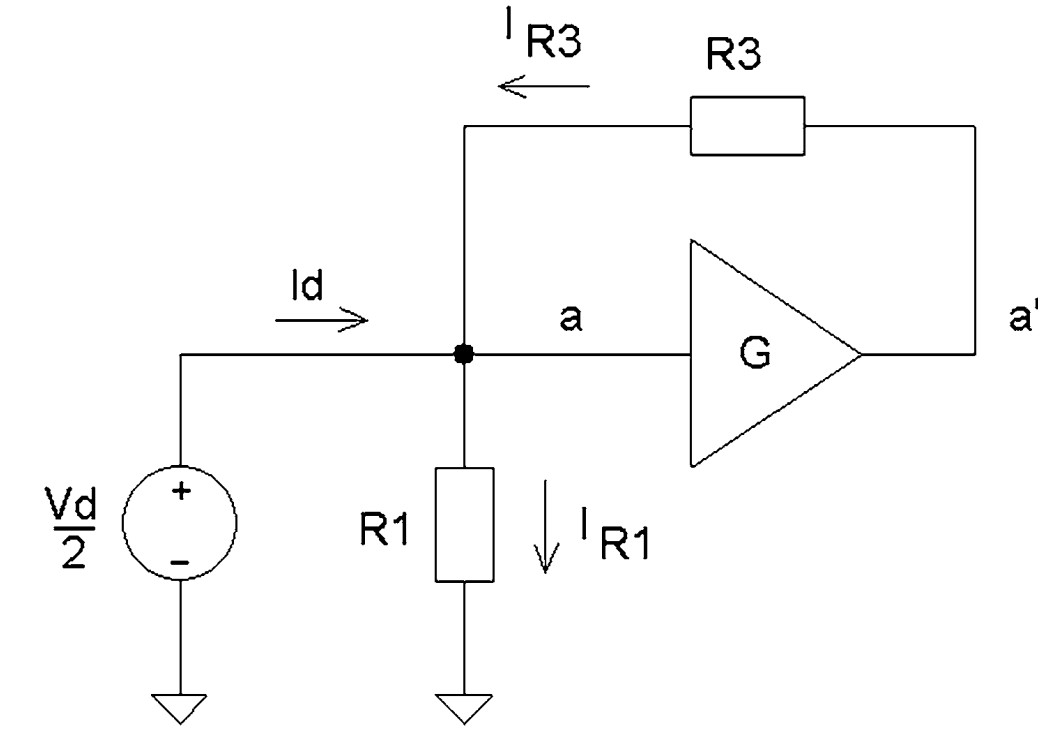
\includegraphics[width=0.9\textwidth]{images/diff_half}
		\caption{Half-circuit equivalent scheme}
		\label{fig:half_circuit_equivalent}
	\end{subfigure}
	\caption{Differential Mode Analysis}
	\label{fig:differential_analysis}
\end{figure}

The differential resistance \(R_d\) is calculated by:
\begin{equation}
	R_d = \frac{V_d / 2}{I_d}
	\label{eq:diff_resistance}
\end{equation}

Applying Kirchhoff's Current Law (KCL) at node a:
\begin{equation}
	I_d = I_{R1} - I_{R3}
	\label{eq:kcl}
\end{equation}
where:
\begin{equation}
	I_{R1} = \frac{V_d / 2}{R_1}
	\label{eq:ir1}
\end{equation}
and:
\begin{equation}
	I_{R3} = \left( \frac{G \cdot V_d / 2 - V_d / 2}{R_3} \right) = \left( \frac{V_d / 2}{R_3} \right) \cdot (G - 1)
	\label{eq:ir3}
\end{equation}
Thus:
\begin{equation}
	I_d = \frac{V_d / 2}{R_1} - \left( \frac{V_d / 2}{R_3} \right) \cdot (G - 1)
	\label{eq:id}
\end{equation}

Substituting \(I_d\) in the \(R_d\) equation gives:
\[
R_d = \frac{V_d / 2}{V_d / 2 \left[ \frac{1}{R_1} - \frac{(G - 1)}{R_3} \right]}
\]
\[
\frac{1}{R_d} = \frac{1}{R_1} - \frac{(G - 1)}{R_3}
\]
\begin{equation}
	R_d = \frac{R_1 R_3}{R_1 + R_3 - R_2}
	\label{eq:rd}
\end{equation}

In the equation \eqref{eq:rd}, the differential input resistance \(R_d\) can be infinite if the value of \(R_2\) equals the sum of \(R_3\) and \(R_1\):
\begin{equation}
	R_2 = R_3 + R_1
	\label{eq:r2}
\end{equation}

Considering resistor tolerances, which affect differential input resistance, the worst-case differential resistance can be estimated by including a tolerance factor \(\delta\):
\begin{equation}
	R_d \approx \frac{R_1 \parallel R_3}{\delta}
	\label{eq:tolerance}
\end{equation}
where \(\delta\) is the tolerance percentage.

For simplicity, assuming \(R_1 = R_3 = R\):
\begin{equation}
	R_d \approx \frac{R}{2\delta}
	\label{eq:simple_rd}
\end{equation}

For a tolerance (\(\delta\)) of 1\% and \(R = 1 \text{M}\Omega\):
\begin{equation}
	R_d = 50 \text{M}\Omega
	\label{eq:final_rd}
\end{equation}

This analysis shows that worst-case differential resistance is sufficiently high. 



\item \textbf{Common Mode Analysis}

Similar to differential mode analysis, a simplified version of the front-end circuit with a common voltage source is depicted in Figure \ref{fig:common_mode_simplified}. In the half-circuit equivalent Figure \ref{fig:common_mode_half_circuit}, the gain coefficient sign is not inverted as connecting \(R_3\) to its opposite op-amp input is equivalent to connecting it to its corresponding input because both op-amps receive the same common mode input signal.

\begin{figure}[h]
	\centering
	\begin{subfigure}{0.5\textwidth}
		\centering
	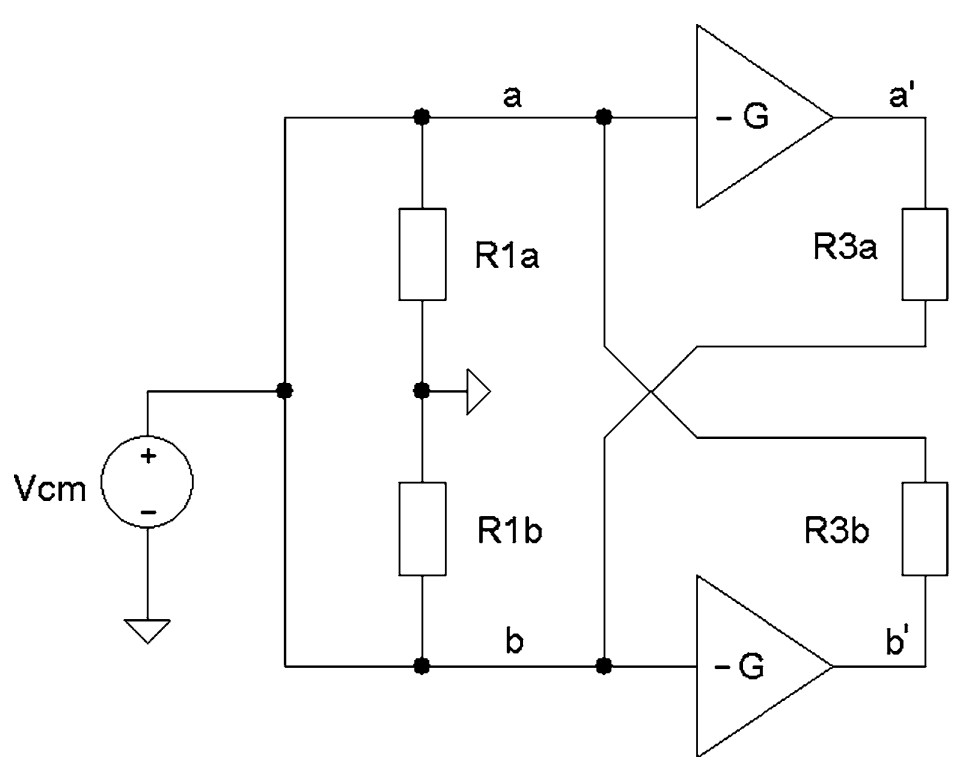
\includegraphics[width=0.8\textwidth]{images/common mode simplified}
		\caption{Simplified Common Mode Equivalent Circuit}
		\label{fig:common_mode_simplified}
	\end{subfigure}
	\hfill
	\begin{subfigure}{0.4\textwidth}
		\centering
		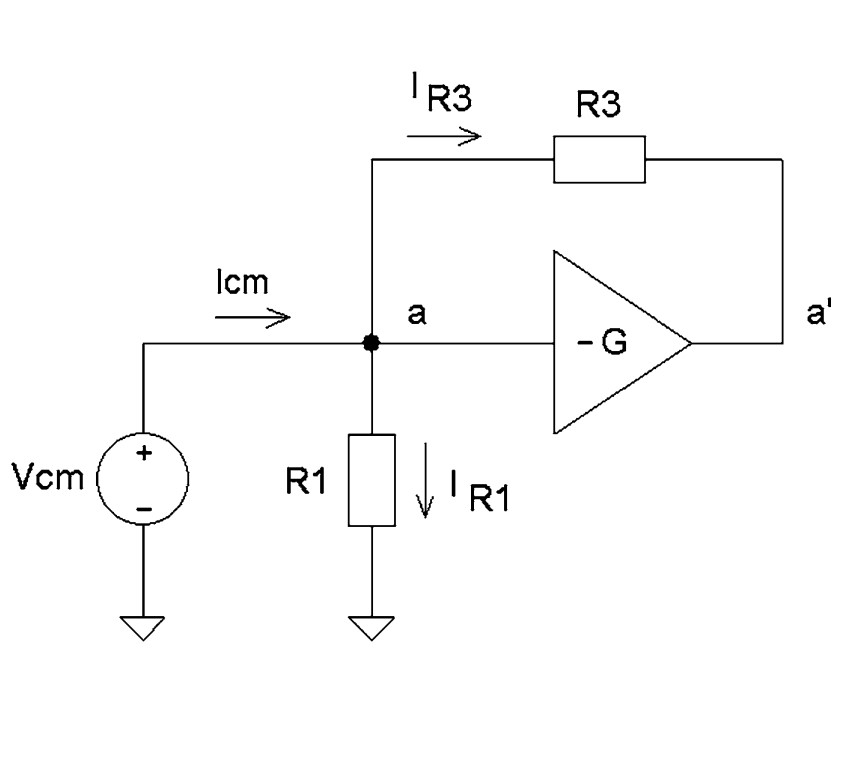
\includegraphics[width=0.9\textwidth]{images/common mode half}
		\caption{Half-Circuit Equivalent Scheme}
		\label{fig:common_mode_half_circuit}
	\end{subfigure}
	\caption{Simplified and Half-Circuit Equivalent Schemes for Common Mode Analysis}
	\label{fig:common_mode_analysis}
\end{figure}

As illustrated in Figure \ref{fig:common_mode_analysis}, the common mode resistance \(R_{cm}\) is calculated as follows:
\begin{equation}
	R_{cm} = \frac{V_{cm}}{I_{cm}}
	\label{eq:rcm}
\end{equation}

Applying Kirchhoff's Current Law (KCL) at node 'a':
\begin{equation}
	I_{cm} = I_{R3} + I_{R1}
	\label{eq:icm_kcl}
\end{equation}
where:
\begin{equation}
	I_{R1} = \frac{V_{cm}}{R_1}
	\label{eq:ir1_cm}
\end{equation}
and:
\begin{equation}
	I_{R3} = \frac{V_{cm} - (-G \cdot V_{cm})}{R_3} = \frac{V_{cm}(1 + G)}{R_3}
	\label{eq:ir3_cm}
\end{equation}

Substituting into the expression for \(I_{cm}\):
\begin{equation}
	I_{cm} = \left( \frac{V_{cm}}{R_1} \right) + \left( \frac{V_{cm}(1 + G)}{R_3} \right)
	\label{eq:icm}
\end{equation}
\begin{equation}
	I_{cm} = V_{cm} \left( \frac{1}{R_1} + \frac{1 + G}{R_3} \right)
	\label{eq:icm_simplified}
\end{equation}

Substituting this into the expression for \(R_{cm}\):
\begin{equation}
	\frac{1}{R_{cm}} = \frac{1}{R_1} + \frac{1 + G}{R_3}
	\label{eq:rcm_inverse}
\end{equation}
\begin{equation}
	R_{cm} = \frac{R_1 R_3}{R_1 + R_3 + G R_1}
	\label{eq:rcm_final}
\end{equation}
Substituting eg.\ref{eq:gain} in the above expression gives
\begin{equation}
	R_{cm} = \frac{R_1 R_3}{R_1 + R_3 + R_2}
	\label{eq:rcm_r2}
\end{equation}
\begin{equation}
	R_{cm} = \frac{R_1 R_3}{2 (R_1 + R_3)} = \frac{R_1 \parallel R_3}{2}
	\label{eq:rcm_parallel}
\end{equation}

The common mode resistance per both inputs will be:
\begin{equation}
	R_{CM} = \frac{R_{cm}}{2} = \frac{R_1 \parallel R_3}{4}
	\label{eq:rcm_per_input}
\end{equation}

If \(R_1 = R_3 = 1 \text{M}\Omega\):
\begin{equation}
	R_{CM} = \frac{R}{8} = \frac{1 \text{M}\Omega}{8} = 125 \text{k}\Omega
	\label{eq:final_rcm}
\end{equation}

This analysis confirms that the differential input resistance is very high, while the common mode resistance is sufficiently low.

\item \textbf{Component Selection}

Selecting the right components is crucial for the front-end circuit to ensure consistent treatment of both ECG electrodes. It is desirable to use a dual I/O package op-amp to maintain symmetry. Additionally, the op-amp should have a low quiescent current to minimize power consumption, essential for battery-powered applications. The OPA2338 was selected for this purpose; it is a dual CMOS op-amp that offers low cost, miniature size, high gain bandwidth product of 3MHz, and a low quiescent current of 525 µA, making it well-suited for ECG acquisition on battery power \cite{TI_OPA2338_datasheet}.


\end{itemize}

\subsubsection{Protection Circuit}
\vspace{1em}
The ECG circuit, designed to operate on a DC 3.7V battery, is inherently isolated from AC mains, necessitating specific measures for protection against overvoltage and electrostatic discharge (ESD). These protections are critical as ESD can transfer to the ECG circuit from the human body, potentially causing permanent damage.\\

\begin{itemize}
\item \textbf{Overvoltage Protection}

To safeguard against overvoltage, each electrode of the ECG is equipped with a Zener diode configured for a Zener breakdown voltage \( V_z = 3.6V \). This setup forms a double-clipping Zener diode circuit, as illustrated in Figure \ref{fig:overvoltage_protection}. Under normal conditions, where the electrode line voltage remains below \( V_z \) (Zener forward voltage), the Zener diodes do not conduct any current. However, if an overvoltage occurs, such as an electrode 'R' exceeding \( 3.6V + V_f \) (the forward voltage drop), the corresponding Zener diode \( Z1 \) becomes forward biased, and \( Z2 \) reverse biased, effectively clamping the electrode 'R' line voltage at \( 3.6V + V_f \). The PN-MM3Z3V6T1G was selected for its low Zener reverse leakage current of 5μA \cite{Mouser_MM3Z2V4T1_datasheet}.

\item \textbf{ESD Protection}

For ESD protection, a 3-pin steering diode is employed on each electrode line, as depicted in Figure \ref{fig:esd_protection}. This steering diode configuration uses two diodes stacked with the cathode of one connected to the anode of the other, providing connections at the cathode, anode, and the midpoint between the two diodes. The BAV99 diode was chosen due to its high switching speed, low capacitance, and substantial breakdown voltage. As shown in Figure \ref{fig:esd_protection}, during high transient ESD events, the diode \( D1 \) becomes forward-biased, allowing the ESD signal to be diverted to the ground via a decoupling capacitor linked to the power line, effectively protecting the circuit from ESD-induced damage.
\end{itemize}

\begin{figure}[h]
	\centering
	\begin{subfigure}{0.45\textwidth}
		\centering
		\includestandalone{standalones/Circuits/overvoltage}
		\caption{Illustration of Overvoltage Protection Circuit}
		\label{fig:overvoltage_protection}
	\end{subfigure}
	\hfill
	\begin{subfigure}{0.45\textwidth}
		\centering
		\includestandalone{standalones/Circuits/esd}
		\caption{Configurations of Steering Diode During ESD Protection}
		\label{fig:esd_protection}
	\end{subfigure}
	\caption{Overall Protection Circuit: Overvoltage and ESD Protection}
	\label{fig:protection_circuit}
\end{figure}

\noindent Figure \ref{fig:protection_circuit} illustrates the overall protection circuit configurations for overvoltage and ESD protection, redrawn from \cite{TI_SLVA898}.//

\subsubsection{High Pass Filter Design}
\vspace{1em}
To address the low-frequency noises present in the ECG signal, which were detailed in Section \ref{noises}, a passive high-pass filter was designed for integration at each ECG electrode input prior to the differential amplifier stage as shown in Figure \ref{fig:high_pass_filter}. The primary noises targeted by this filter include baseline wander and motion artifacts, which typically range from 1 to 10 Hz but are most dominant between 1 to 5 Hz. Consequently, the high-pass filter was designed to have a cutoff frequency slightly above this range, at 6 Hz, to ensure effective noise mitigation.

\begin{figure}[h]
	\centering
	\includestandalone{standalones/filter/high pass}
	\caption{Passive High Pass Filter Circuit}
	\label{fig:high_pass_filter}
\end{figure}

\noindent The cutoff frequency for a passive high-pass filter is determined by the formula:
\[ F_c = \frac{1}{2\pi RC} \]

\noindent For this design, resistors \( R1 \) and \( R2 \) were set at 27kΩ, and capacitors \( C1 \) and \( C2 \) at 1µF. These component values yield a cutoff frequency (\(-3\) dB point) of the filter calculated as follows:
\[ F_c = \frac{1}{2\pi \times 27000 \times 0.000001} = 5.89 \text{ Hz} \]

\noindent The behavior of this filter at various frequencies is illustrated in the Bode plot shown in Figure \ref{fig:bode_plot_high_pass}. This plot provides a visual representation of the filter's effectiveness in attenuating frequencies below 5.89 Hz, thereby enhancing the overall signal quality of the ECG by reducing the impact of low-frequency noise.\\

\begin{figure}[h]
	\centering
	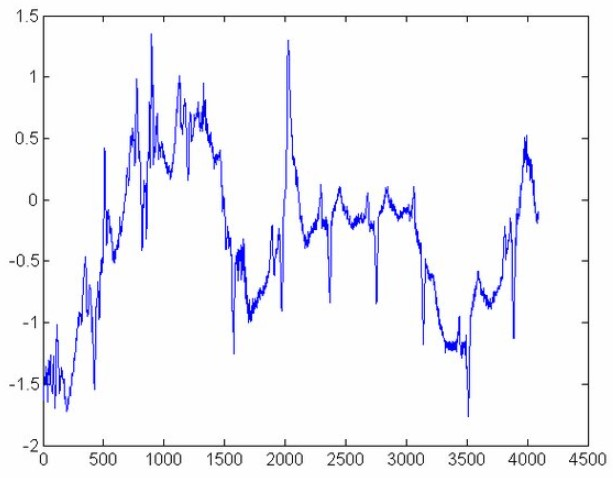
\includegraphics[width=0.6\textwidth]{images/motionArtifacts}
	\caption{Bode Plot of High-Pass Filter}
	\label{fig:bode_plot_high_pass}
\end{figure}

\noindent This high-pass filter design is crucial for improving the clarity and accuracy of the ECG readings by effectively filtering out undesirable low-frequency components before further amplification and processing.\\

\subsubsection{Differential Amplifier}
\vspace{1em}
Based on the principles of the Einthoven triangle described in Section {einthoven}, the potential difference between the left and right limbs yields the resultant ECG signal for that particular lead. To capture this potential difference, differential amplifiers are typically employed in analog electronics. Given that ECG signals have amplitudes of less than 5mV, amplification is essential for better visualization and feature extraction. \\

\noindent While a non-inverting amplifier with an appropriate gain could be used in series with the differential amplifier to serve both amplification and differential purposes, mismatches in feedback resistors for each electrode line could lead to significant signal discrepancies when amplified. This would adversely affect the output from the differential amplifier. To overcome this issue, an instrumentation amplifier is employed, enhancing signal integrity and consistency.

\begin{figure}[h]
	\centering
	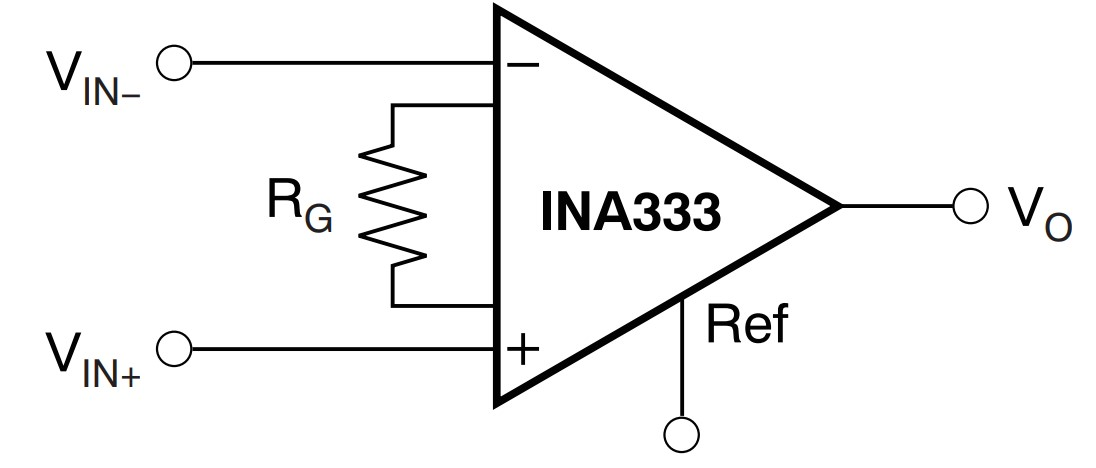
\includegraphics[width=0.6\textwidth]{images/Instrumentational amplfier}
	\caption{Illustration of Instrumentation Amplifier Setup}\cite{TI_INA333}
	\label{fig:instrumentation_amplifier}
\end{figure}

\noindent For this project, the instrumentation amplifier PN-INA333 \cite{TI_INA333} was chosen due to its precision-matched internal feedback resistors. An external resistor \( R_G \) allows for adjustable gain, calculated as:
\begin{equation}
G = 1 + \left(\frac{100k}{R_G}\right)
	\label{eq:gain equation}
\end{equation}

\noindent For the thesis, \( R_G = 1.01k \) was selected, achieving a desired gain of 100. This instrumentation amplifier provides a high Common Mode Rejection Ratio (CMRR) of 100 dB for gains greater than 10, which is crucial for minimizing common mode noise further, in addition to the front-end circuit's contribution. Its low quiescent current of 50µA makes the INA333 particularly suitable for battery-powered applications.\\

\noindent The INA333 also features a reference pin that adds flexibility for DC biasing the ECG signal. Since the circuit operates on a single 0 to 3.3V rail, to prevent the clamping of the negative part of the ECG signal, this signal is biased to Vcc/2 (1.65V) using the reference pin. According to the datasheet \cite{TI_INA333}, to preserve the CMRR value of the amplifier, the reference pin should have an external impedance of less than 15 ohms. To meet this requirement, an external voltage reference IC, PN-REF2033 \cite{TI_REF2033}, is used. This component provides a stable, low-drift, low-noise, low-impedance 1.65V reference voltage, operating at a quiescent current of 360µA.\\







		%Methods
	%
	%How is the approach implemented and checked?
	%All necessary information for the reproduction
	%% !TeX root = ../thesis.tex

\ifgerman{\chapter{Methoden}}
\ifenglish{\chapter{Methods}}

	
	%Results
	%
	%Well, does it work?
	%Results of measurements/simulations etc.
	% !TeX root = ../thesis.tex

\ifgerman{\chapter{Ergebnisse}}
\ifenglish{\chapter{Results}}

	
	%Discussion
	%
	%How to interpret the results?
	%Discussion of successes, limitations and explanatory approaches
	%Next steps to be taken
	% !TeX root = ../thesis.tex

\ifgerman{\chapter{Diskussion}}
\ifenglish{\chapter{Discussion}}

\ifgerman{\section{Zusammenfassung}}
\ifenglish{\section{Summary}}

\ifgerman{\section{Ausblick}}
\ifenglish{\section{Outlook}}

	
	
	%%Introduction to LaTeX
% !TeX root = ../thesis.tex

\chapter{BaMa Template}

\section{\LaTeX~Basics}

LaTeX uses source code which is compiled to generate documents. This has several advantages when creating large documents: 

\begin{itemize}
	\item Separation of template and document possible
	\item Consistent text format across sections and documents oriented at norms like DIN~1450
	\item Customisable and reproducible generation of table of contents, figures and index
	\item Automation of tasks like number formatting, plot generation, \dots
	\item Inclusion of external files like measurement data without the need for copy and paste
	\item Automated tasks like number formatting 
\end{itemize}

\subsection{Command syntax}

LaTeX commands have the following syntax:

\begin{lstlisting}
	\command[options]{argument}
\end{lstlisting}

There are also environments which can be opened and closed:

\begin{lstlisting}
	\begin{environmentname}
		...
	\end{environmentname}
\end{lstlisting}

As the backslash is used as prefix for commands and the percent sign for commands a few escape sequences are necessary as listed in table~\ref{tab:escseq}. For more special characters see \url{http://detexify.kirelabs.org/classify.html}.

\begin{table}[H]
	\centering
	\caption{\LaTeX escape sequences}
	\label{tab:escseq}
	\begin{tabular}{ccc}
		\toprule
		Sign & \LaTeX special meaning  & Escape sequence\\
		\midrule
		\textbackslash~(backslash) & command initializer & \verb|\textbackslash| \\
		\%~(percent) & comment for rest of line & \verb|\%| \\
		\textasciitilde~(tilde) & line break protected space & \verb|\textasciitilde| \\
		\$~(dollar sign) & start math mode & \verb|\$| \\			
		\bottomrule
	\end{tabular}
\end{table}

\subsection{Main document structure}

Documents normally have the following components:

\begin{itemize}
	\item \verb|\documentclass[options]{classname}|: Loads the documents template which defines the appearance like article, conference paper, \dots. The bama template uses a custom class located in the main directory of the repository.
	\item \verb|\usepackage[options]{packagename}|: Loads packages for additional capabilities. More information about packages is available at ctan \footnote{\url{https://www.ctan.org/}}.
	\item \verb|\input{filename}|: Inserts the content of another \TeX file \footnote{include serves a similar purpose, has more restrictions but offers  higher compilation speeds.}.
	\item The content of the document in between \verb|\begin{document}| and \verb|\end{document}|
\end{itemize}

\subsection{Heading structure}

There are several levels of headings which are listed in the following. Avoid having a single heading of a certain hierarchy e.g. if there is section 1.1 there should also be at least 1.2.

\begin{description}
	\item [part] is the highest hierarchy. Parts have big headings occupying a whole page. It is not needed for the thesis.
	\item [chapter] is a high hierarchy heading causing page breaks to next uneven page. It is not available in all classes but should be used for the thesis.
	\item [section] is used to separate chapters. One can also use \verb|\subsection| and \verb|\subsubsection| for further hierarchy levels.
	\item [paragraph] and \verb|\subparagraph| are used for small passages and do not cause a line break after the heading.
\end{description}

\subsection{Text formatting}

LaTeX distinguishes between line break and paragraph. Do not use the line break operator for paragraphs, just insert an empty line in the source code. Sometimes special formatting is useful e.g. to center figures but manual font size and style changes in normal text should be avoided.

\begin{table}[H]
	\centering
	\caption{Text formatting}
	\label{tab:textformat}
	\begin{tabular}{ccc}
		\toprule
		Feature & command\\
		\midrule
		Line break & \verb|\\| \\
		Paragraph & empty line in code \\
		\textit{italic} & \verb|\textit{...}| \\
		\textbf{bold} & \verb|\textbf{...}| \\
		center & \verb|\centering| \\	
		\bottomrule
	\end{tabular}
\end{table}

\subsection{Dashes}

\begin{table}[H]
	\centering
	\caption{Dashes}
	\label{tab:dashes}
	\begin{tabular}{cccc}
		\toprule
		Name & Code & Example & Usage\\
		\midrule
		dash & \verb|-| & - & hyphen\\
		Viertelgeviertstrich & &  & Binde-, Trennungs-, Ergänzungsstrich\\
		en dash & \verb|--| & -- & number range\\
		Halbgeviertstrich & & & Gedanken-, Bis-strich, bei Geldbeträgen\\
		em dash & \verb|---| & --- & parenthetic expression \\
		Geviertstrich &  & & Spiegelstrich\\
		%Doppelgeviertstrich & \verb|--\,--| & --\,-- & Zensurstrich (englisch)
		\bottomrule
	\end{tabular}
\end{table}

Hyphens are automatically inserted to break lines and achieve justification. Although the corresponding parameters should be set correctly special words can lead to problems. For example MUSIC-Alogrithmus has a dash which means that hypens at other places are not allowed. This can be prevented by the syntax \hbox{\verb|MUSIC-Algo\-rithmus|} which allows an optional line break. The same problems can occur due to protected whitespaces.

\subsection{Lists}

There are two major list types in {\LaTeX}: numerated (\texttt{enumerate}) and not numerated (\texttt{itemize}). Furthermore there is the type \texttt{description} for explaining keywords. Lists are started with \texttt{begin} and stopped with \texttt{end}. They can also be nested.

\begin{enumerate}
	\item High level with numbering
	\begin{itemize}
		\item Detailed information
		\item without numeration
	\end{itemize}
	\item Another big point
	\item \dots and more
\end{enumerate}

\begin{lstlisting}[language=TeX]
\begin{enumerate}
	\item High level with numbering
	\begin{itemize}
		\item Detailed information
		\item without numeration
	\end{itemize}
	\item Another big point
	\item \dots and more
\end{enumerate}
\end{lstlisting}

\section{Math mode and Numbers}

	Normaly LaTeX operates in text mode, but for expressions like $x=5$ the math mode can be activated and deactivated using \verb|$|. In math mode text is italic and exhibits changed letter spacing.
	
	For indexed equations the \verb|equation| environment is suited when using vanilla LaTeX. With the package \verb|amsmath| the \verb|align| environment is available which is recommended here:
	
	\begin{align}
		\label{eq:alignDemo}
		\oint_{\partial A} \vect{B}_\text{ind} \dd{\vect{l}} &= \mu_0 \left( \iint_A \vect{j}_\text{ind} \dd{\vect{A}} + \varepsilon_0 \frac{\partial}{\partial t} \iint_A \vect{E} \dd{\vect{A}} \right) \\
		\text{und außerdem} \nonumber \\
		\label{eq:alignDemo2}
		Q &= \oiint_A \vect{D} \dd{\vect{A}} = \iiint_V \rho_{\text{Volumen}} \dd{V}
	\end{align}
	
	\begin{lstlisting}[language=TeX]
	\begin{align}
	\label{eq:alignDemo}
	\oint_{\partial A} \vv*{B}{\text{ind}} \dd{\vv{l}} &=
		\mu_0 \left( \iint_A \vv*{j}{\text{ind}} \dd{\vv{A}}
		+ \varepsilon_0 \frac{\partial}{\partial t} \iint_A \vv{E} \dd{\vv{A}} \right) \\
	\text{und außerdem} \nonumber \\
	\label{eq:alignDemo2}
	Q &= \oiint_A \vv{D} \dd{\vv{A}} = \iiint_V \rho_{\text{Volumen}} \dd{V}
	\end{align}
	\end{lstlisting}

	Equations can be easily referenced when the package \verb|mathtools| is used by the the command \verb|\eqref{eq:alignDemo}| (e.g. Eq.~\eqref{eq:alignDemo}).
	
	Between numbers and units a half length space has to be inserted (\verb|\,|) \footnote{For details see DIN~1338}. In German a comma has to be used instead of a dot. The package \verb|siunitx| can handle the correct formatting of numbers with units. The syntax is showed in table~\ref{tab:numberUnitFormat}. Also note that in German the letter \enquote{$U$} is used for voltage instead of \enquote{$V$}.
	
	\begin{table}
		\centering
		\caption{Number- and Unit formatting}
		\label{tab:numberUnitFormat}
		\begin{longtable}{p{.25\textwidth}p{.1\textwidth}p{.1\textwidth}p{.4\textwidth}}
			\toprule
			Variables & \textit{italic} & $x$\newline $y$\newline $f$\newline $\omega$ & \verb|$x$|\newline \verb|$y$|\newline \verb|$f$|\newline \verb|$\omega$|\\
			Scientific constants & \textit{italic} & $c_0$\newline $\mu_0$\newline $\varepsilon_0$ & \verb|$c_0$|\newline \verb|$\mu_0$|\newline \verb|$\varepsilon_0$|\\
			Units & upright & \si{\milli\ampere}\newline $\SI{3.0}{\micro\metre}$\newline \SI{1.41}{} & \verb|\si{\milli\ampere}|\newline \verb|$\SI{3.0}{\micro\metre}$|\newline \verb|\SI{1.41}{}|\\
			Operators & upright & $\frac{\dd{x}}{\dd{y}}$\newline $\sin$\newline $\cos$\newline $\arg$ & \verb|$\frac{\dd{x}}{\dd{y}}$|\newline \verb|$\sin$|\newline \verb|$\cos$|\newline \verb|$\arg$|\\
			Mathematic constants & upright & $\ee$\newline $\ii$\newline $\jj$\newline $\pipi$ & \verb|$\ee$|\newline \verb|$\ii$|\newline \verb|$\jj$|\newline \verb|$\pipi$| \\
			\bottomrule
		\end{longtable}
	\end{table}

	\section{Floating environments}
	\label{sec:floatenvironments}
	
		Floating objects are objects whose position in the final document can depart from the source code. The most common floating objects are figures and tables. Commonly they are placed at the top or bottom of a page to not split the text apart and make reading more pleasant. Floats can also be longer than a single page.
		
		Floats are created by using \verb|\begin{figure}| / \verb|\end{figure}| for figures and \verb|\begin{table}| / \verb|\end{table}| for tables. The content is defined in between and can be arbitrarily chosen. Floats should have a meaningful caption which is specified with \texttt{{\textbackslash}caption[register entry]\{caption text\}}. The command \texttt{{\textbackslash}label} is used to enable referencing them.
		
		Sometimes {\LaTeX} has troubles to determine the best position for a float. In these cases optional arguments or packages like \texttt{placeins} can be used.
		
		\begin{itemize}
			\item t (top, top of page)
			\item b (bottom, bottom of page)
			\item p (page, on an individual page)
			\item h (here, exactly at this position)
			\item H (HERE, forced to place exactly at this position (provided by the package \texttt{float})
		\end{itemize}
		
		As the options are not enforced one can add a second priority \verb|\begin{figure}[tb]|. The only enforced option is \enquote{H}.

		Instead of forced positioning the float environment can also be skipped and the caption with \texttt{{\textbackslash}captionof\{figure/table\}[register entry]\{caption text\}} added.
		
		\paragraph{Labels and References}
		
		Floating elements are commonly labeled using a \texttt{label} which is issued after the caption. It is recommended to add the type of object e.g. \verb|\label{eq:maxwell}|, \verb|\label{fig:blockDiagramTx}|. Labels can also be created for sections, subsections, \dots.
		The labels can be references using \verb|\ref{fig:blockDiagramTx}|. Only the number is output so you have to add the type manually e.g. \verb|see figure~\ref{fig:blockDiagramTx} and equation~\eqref{eq:maxwell}|. It will look like this figure~\ref{fig:tikz}. The page can be found with \verb|\pageref|. Multiple compilations are required until all references are correctly included in the document.
		
		\paragraph{Caption}
		
		Always choose a meaningful caption for floats, especially if they are not directly placed at the text section. If figures are included from other documents always add a citation to the caption.
	
	\subsection{Figures}
	\label{sec:figures}
	
		\subsubsection{External Graphics}
			
		Graphics can be included using the package \texttt{graphicx} as it is done on the title page. Vector graphics are recommended over pixel graphics. They can be included in the format pdf. The include command is \verb|\includegraphics[width=.8\textwidth]{imagefile}|. Alternatively the height can be specified and also given in cm.
		
		\begin{lstlisting}[language=TeX]
			\begin{figure}[tb]
				\centering
				\includegraphics[width=.8\textwidth]{images/receiverChain}
				\caption{Description and then references \cite{BibDEMO1, BibDEMO2, BibDEMO3}}
				\label{fig:receiverChain}
			\end{figure}
		\end{lstlisting}
	
		\subsubsection{Tikz and Circuitikz}
		
		Tikz is a package based on pgf and allows to draw graphics using lines, rectangles, polygons and so on. There is also a further extension called Circuitikz which allows to draw schematics and also has been enhanced by \acs{LTE}.
		
		There are several approaches to avoid long compilation times when drawing a new graphic:
		
		\begin{itemize}
			\item Develop the graphic using KtikZ resp. QtikZ and paste it into the thesis
			\item Use tikz externalize to save compiled graphics automatically in external files
			\item Use standalone class to create a separate document for the graphic. The {\TeX} is later imported to the main document.
		\end{itemize}
	
		For this template the later option is chosen because it has the additional advantage that graphics can be reused in further documents like papers or presentations. Required packages for the external graphics can be loaded in one of the header files and included in both documents. The filter in Figure~\ref{fig:tikz} is used as an example for this method.
		
		\begin{lstlisting}[language=TeX]
		\begin{figure}
			\centering
			\includestandalone{standalones/filter/filter}
			\caption{Schaltplan einer Operationsverstärkerschaltung, erstellt in circuitikz mit Hilfe der Entwicklungsumgebung QTikZ}
			\label{fig:tikz}
		\end{figure}.
		\end{lstlisting}
		
		\begin{figure}
			\centering
			\includestandalone{standalones/filter/filter}
			\caption{Schaltplan einer Operationsverstärkerschaltung, erstellt in circuitikz mit Hilfe der Entwicklungsumgebung QTikZ}
			\label{fig:tikz}
		\end{figure}
	
		\subsubsection{Styling of Plots}
		
		Plots are a common element of a thesis. In order to achieve high quality plots they can be directly generated using {\TeX} or imported using a suited vector graphic format.
		
		Scientific plots have to be labelled correctly. Only the following formats are allowed. The space before and after \enquote{in} / the slash can vary.
		
		\begin{enumerate}
			\item $E${\qquad}in{\qquad}\si{\volt\per\meter}
			\item $E$ / (\si{\volt}/\si{\meter})
		\end{enumerate}
	
		\subsubsection{pgfplots}
		
		Plots from expressions, measured or simulated data can be directly plotted using the famous \texttt{pgfplots} package. An example for an expression is given in Figure~\ref{fig:parabelpgf}.
		
		\begin{figure}[h]
			\centering
			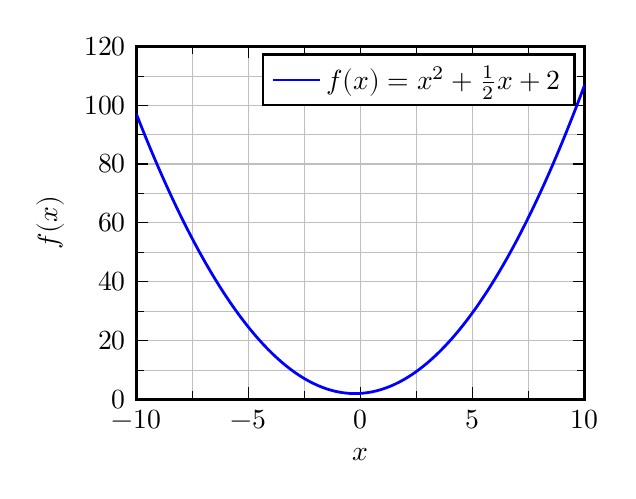
\begin{tikzpicture}
				\begin{axis}[
					width=.6\textwidth,
					height=.5\textwidth,
					domain=-10:10,
					xmin=-10, xmax=10,
					ymin=0, ymax=120,
					samples=100,
					ytick distance = 20,
					minor tick num = 1,
					%grid = both,
					%title = {\textbf{Parabelplot mit TikZ}},
					xlabel = {$x$},
					ylabel = {$f(x)$},
					legend entries = {$f(x) = x^2 + \frac{1}{2}x + 2$},
					]
					\addplot+[mark=none] {x^2 + 0.5*x + 2};
				\end{axis}
			\end{tikzpicture}
			\caption{Example plot for an expression using pgfplots}
			\label{fig:parabelpgf}
		\end{figure}
	
		Another, more advanced example is given in Figure~\ref{fig:sparameterpgf}. It uses a 2-port S-Parameter file to plot the input reflection in a smith chart and also reflection and transmission in a linear plot. The diagrams are created in a separate file using standalone. Also note that the package \texttt{subcaption} is used to create subplots.
	
		\begin{figure}[h]
			\centering
			\begin{subfigure}{0.75\textwidth}
				\centering
				\includestandalone{standalones/sparameter/sparameterSmith}
				\caption{Smith Chart plot}
			\end{subfigure}
			\\
			\begin{subfigure}{0.75\textwidth}
				\centering
				\includestandalone{standalones/sparameter/sparameter}
				\caption{}
			\end{subfigure}
			\caption{S-Parameter of a filter created on the website \url{https://rf-tools.com}}
			\label{fig:sparameterpgf}
		\end{figure}
		
		\subsubsection{Matlab plots}
		
		To avoid the use of pixel graphics there exist tools like \texttt{matlab2tikz}\footnote{\url{https://github.com/matlab2tikz/matlab2tikz}}. It is recommended to use such a tool to generate high quality plots with a consistent style. \texttt{matlab2tikz} works by generating a \texttt{tex} file from within Matlab. For detailed installation and usage it is referred to the given github repository and the Matlab FileExchange.
		
		A simple example is given below:
		
		\begin{lstlisting}[language=Matlab]
			% generate x and y data
			x=-10:0.1:10;
			y=x.^2 + 1/2*x + 2;
			
			% plotting
			figure(1);
			hold on;
			xlabel('$x$');
			ylabel('$f(x)$');
			plot(x,y,'r')
			legend('$f(x)=x^2 + \frac{1}{2}x + 2$');
			matlab2tikz('pathtotargetfile/matlabtikz.tikz', 'width', '0.5\textwidth', 'parseStrings', false);
		\end{lstlisting}
	
		When previewing graphs in Matlab axis labels appear corrupted because the {\LaTeX} commands are not interpreted in the preview due to the \texttt{parseStrings} option. 
		
		\subsubsection{Python plots using matplotlib}
		
		There are several possibilities to include python plots in {\LaTeX} documents. One of them is the \texttt{pgf} mode of \texttt{matplotlib}. It can be activated with \verb|mpl.use('pgf')| and finally the output can be saved with \verb|plt.savefig("pa2.pgf",bbox_inches='tight')| and \verb|plt.close()|. This method has the advantage that {\LaTeX} expressions inside the graphic are interpreted in the main document allowing i.e. to include cites.
		
		An alternative is \texttt{tikzplotlib} \footnote{\url{https://pypi.org/project/tikzplotlib/}} which allows a more consistent style.
		
	\subsection{Tables}
	
		There are several enhancements for {\LaTeX} tables to improve the default \texttt{tabular} environment. The \texttt{bama} class uses \texttt{longtable} for multi page tables and \texttt{booktabs} for a cleaner design. A simple example is given below:
		
		\begin{lstlisting}[language=TeX]
			\begin{table}
				\centering
				\caption{myTableCaption}
				\label{tab:myTable}
				\begin{longtable}{cc}
					\toprule
					header & second column\\
					\midrule
					content & second column\\
					next row & second column\\
					\bottomrule
				\end{longtable}
			\end{table}
		\end{lstlisting}
	
\section{Lists}

This section refers to lists like the table of contents, list of abbreviations, \dots. These are automatically generated by {\LaTeX}. In order to fully populate them several runs of the compiler may are necessary because the references have to be found in the current run but can not be processed until the next run.

The lists can be generated by the following commands. Some of them are modified by the template in order to provide the required style.

\begin{table}
	\centering
	\caption{Lists of a thesis}
	\label{tab:listofs}
	\begin{tabular}{ll}
		\toprule
		Table of contents:    & {\verb|\tableofcontents|} \\
		List of abbreviations: & {\verb|\printacronyms|} \\
		Bibliography:  & {\verb|\printbibliography|} \\
		List of figures: & {\verb|\listoffigures|} \\
		List of tables:   & {\verb|\listoftables|}\\
		\bottomrule
	\end{tabular}
\end{table}

	\subsection{Abbreviations}
	\label{sec:acronyms}

	Despite a lot of abbreviations are very common in science and engineering the long form of every abbreviation has to be included in the thesis. Therefore there is the package \texttt{acro} which offers the definition of abbreviations in separate file (\texttt{acronyms.tex}) and their use in the document.
	
	\begin{lstlisting}[language=TeX]
	\DeclareAcronym{MOSFET}{
		short = MOSFET,
		long  = Metal-Oxide-Semi\-conductor Field-Effect Tran\-sistor
	}
	\end{lstlisting}

	The abbreviation can be inserted with \verb|\ac{key}| This uses the long form at the first time like \ac{MOSFET} and the short form on the following uses like \ac{MOSFET}.
	
	Long and short forms can also be enforced using \verb|\acl| and \verb|\acs|. Beside that several commands for singular, plural, \dots are available.
	
	Used abbreviations are also included into the list of abbreviations.

	\subsection{Citations}
	\label{sec:literatur}

	Quote worthy literature is cited by the command \verb|\cite| with the literatures key as argument. The style is defined by the template and should by used for a thesis at \acs{LTE} which looks like \cite{BibDEMO1}. Cites can be inserted in the middle of sentences or at the end. Citations at the end of a sentence must be preluded by a space and directly followed by the full stop.
	
	The correct and complete citation of information from literature is absolutely mandatory. A good practice is to insert citations into the caption of figures if they are not created by the author. Referencing common knowledge like Ohm's Law is not necessary.
	
	Bibliography data is stored in bibfiles. There is an entry for every reference.
	
		\begin{verbatim}
		@Article{JassSenBigPaper,
   author  = {Hugh {Jass sen.}},
   title   = {A very-big paper},
   journal = {The journal of very big papers},
   year    = {7991},
   volume  = {MCMXCVII},
		}
		\end{verbatim}
		
		The entry is referred to by the key which is necessary for citing: \verb|\cite{JassSenBigPaper}|. Even before the key is the type of the publication like article, book, conference, online and much more. Additional information is stored according to the chosen type. Depending on the reference type the entry contains different information and looks different in the list of bibliography.
		
		Brackets are used in different places of the entry to avoid wrong wrong formatting. The example uses a bracket to declare \enquote{Jass sen.} as the last name. Otherwise {\LaTeX} would detect \enquote{sen.} as the last name which would lead to an incorrect entry in the list of bibliography.
		
		Luckily the entries rarely have to be created manually. For books the website of the university library\footnote{\url{https://ub.fau.de/}} can serve as a comprehensive source. The entries can also be obtained by the publisher. Citations for papers in electronics engineering can be mostly downloaded from \footnote{\url{https://ieeexplore.ieee.org/}}. To make the job even easier there are numerous tools for managing bibfiles. A common tool is JabRef \footnote{\url{https://www.jabref.org/}} which allows for direct imports from IEEExplore by their number. The automatic formatting generation of citekeys can also be handy. Furthermore JabRef supports the import of metadata from PDFs. Simple drag and drop can be used to import references into JabRef. The current bama template is setup to contain the necessary data.
		
		The entries should contain a unique identifier to yield a useful bibliography. This can be the ISBN for books like \cite{tietze2019} or the DOI for digital formats like \cite{paskin1999}. The corresponding url is automatically inserted as invisible link into the bibliography.
		
		Less scientific works can be described by the type \texttt{TechReport} or \texttt{online} like \cite{stm32l476, lehman2020}. These often do not contain a single author which is ok, but it has to be made sure that the reference can be found e.g. by giving a revision number.
		
		The inclusion of bibliography data is not done by {\LaTeX} itself but the a bibliography backend. In this template \texttt{biber} is used which generates a file that is included in additional runs of {\LaTeX}. This mechanism is the reason why several iterations are necessary to fully populate the bibliography.

	\section{Source Code}

		Code can be included by the environment \texttt{lstlisting}. Code can be directly inserted by the following command.
		
		\lstnewenvironment{lstlistingoflisting}
		{\lstset{language=TeX}}
		{}
		\begin{lstlistingoflisting}[language=TeX]
			\begin{lstlisting}[language=C]
				#include<stdio.h>
				
				int main(void) {
					printf("Hallo Welt"); // comment (Test for special chars: äöüß)
					return 0;
				}
			\end{lstlisting}
		\end{lstlistingoflisting}
	
		yielding

		\begin{lstlisting}[language=C]
			#include<stdio.h>

			int main(void) {
				printf("Hallo Welt"); // comment (Test for special chars: äöüß)
				return 0;
			}
  		\end{lstlisting}

		Code can also be read in form files with \texttt{firstline} and \texttt{lastline} specifying the used part of the file. \texttt{firstnumber} is the first number on the left side of the code block.
		
		\begin{lstlisting}[language=C]
			\lstinputlisting[language=C, firstline=15, lastline=17, firstnumber=15]{code/codeexample.c}
		 \end{lstlisting}
		
	\section{Indices\index{Indices}}
	
		{\LaTeX} also supports the creation of indices but it has been removed from the template due to the seldom use. It can be added with the package \texttt{imakeidx}. It supports simple indice \verb|\index{indice}| and sub-indices \verb|\index{indice!subindice}|. It is necessary to also execute \textit{makeindex} in a similar fashion than the bibliography.

	\section{Why Lua{\LaTeX}?}
	
		Lua{\LaTeX} supports additional features compared to pdflatex like direct entering of \enquote{°}, \enquote{µ} and umlaut in the code. It is also possible to execute scripts like outputting the value of $\pipi = \SI{\directlua{tex.print(math.pi)}}{}$ or the generation of PDF metadata from user variables.
		
	\section{Additional packages}
	
	Feel free to modify the files in the \texttt{header} folder to include further packages if you have additional needs like making notes with the \texttt{ToDoNotes} package which allows inserting colourful notes that can be hidden with one switch.
	
	If you have found an improvement to basic settings and packages please let the maintainer of the template know in order to improve the template.

\section{Troubleshooting}
\label{sec:troubleshooting}

	Aside from errors in the source code being one of the top reasons problems can also arise due to outdated files created by the {\LaTeX} Compiler. Deleting auxiliary files, by hand or with the function of TeXstudio, and recompiling the document can solve the problem. Further error sources are listed below.
	
	\begin{itemize}
		\item Outdated packages; {\LaTeX} packages are updated regularly. This can lead to outdated packages of the user which can be resolved by updating or the use of outdated options of the template.
		\item Missing packages; Wrong spelling of commands or using commands of not included packages lead to errors.
		\item Missing or wrong brackets
		\item Environments which do not end or are incorrectly nested.
		\item Using match commands like \verb|\frac| outside of the math mode.
		\item Tables spanning more than one page. This can resolved with the \texttt{longtable} package.
		\item Wrong format of source code files. \enquote{utf8} is recommended.
	\end{itemize}

	Further good practices are:
	\begin{itemize}
		\item Do not change files of the {\LaTeX}-installation. This avoids compilation on other machines.
		\item Do not use absolute paths. This avoids compiling the document on other machines.
	\end{itemize}

	For the most problems there is a lot of information available online. Common and also not that common problems can be found in forums but the package documentations are also pretty helpful.

	%Basics
	%
	%What do you need to know to understand the further chapters
	%All necessary information for understanding the thesis
	%% !TeX root = ../thesis.tex

\ifgerman{\chapter{Grundlagen}}
\ifenglish{\chapter{Basics}}

	
	%State of the art
	%
	%What distinguishes your own approach from the state of the art?
	%Presentation and discussion of the competing solution approaches
	%% !TeX root = ../thesis.tex

\ifgerman{\chapter{Stand der Technik}}
\ifenglish{\chapter{State of the art}}

	

	{\backmatter
		
		% Literatur-, Abbildungs-, Tabellenverzeichnis
		\printbibliography
		\listoffigures
		\listoftables
		
		%if you want to include a cv
		%\include{chapter/cv}
	}
	
	%different section numbering with letters
	\appendix
	
	%appendix content, e.g. long derivations, lots of plots, ...
	\ifgerman{\chapter{Anhang}}
\ifenglish{\chapter{Appendix}}

\section{Close view on details}

	
\end{document}
